\documentclass[a4paper, 12pt]{article}
\usepackage{header_book}

\begin{document}
\titlepage
\thispagestyle{empty}
\pagestyle{fancy}

\newpage
\section*{Предисловие}
Так уж вышло, что предисловие к этой книжке становится в первую очередь послесловием
групп 151 и 153 к нашему лектору. Послесловие --- это всегда грустный жанр, но есть одно
замечательное свойство: послесловия всегда дают надежду на продолжение разговора,
даже если уже много чего было сказано. 

Многие из нас провели с тобой больше года, но все мы надеемся, что всё, что
происходило было не зря в первую очередь для нас. Да, было много трудностей,
которые и мы, и ты преодолевали все 5 модулей. Для тебя мы --- первые студенты,
которых ты учил. Для нас ты первый и, пожалуй, единственный лектор по алгоритмам.

Эта маленькая книжечка не отражает всё, что мы проходили, но в этом модуле были
рассмотрены одновременно практически и теоретически важные алгоритмы.

Мы называли тебя по-сердитому <<Глебас>>, но ты не обижайся, ладно? Отнесись
с юмором :)

Люди, которые прошли все 5 модулей рядом с тобой:

\begin{minipage}{0.45\textwidth}
  \def\baselinestretch{1.2}
  \textbf{Группа 151:}

  \it{

  Бирюков Валентин

  Воробьев Петр

  Калинов Алексей

  Когтенков Алексей

  Корозевцев Павел

  Кутенин Данила

  Лазарев Владислав
  
  Лукьянов Илья

  Мельников Артем

  Мусаткина Дарья

  Проскуряков Александр

  Смалюк Арсений

  Смирнов Александр

  Старченко \sout{Владаимир} Владимир

  Тульчинский Эдуард
  }
\end{minipage}
\hfill
\begin{minipage}{0.45\textwidth}
  \def\baselinestretch{1.2}

  \textbf{Группа 153:}
  \it{

  Абдумуталов Рустам

  Андреев Александр

  Баранов Юрий

  Бесчетнов Павел

  Богомолов Павел

  Гурциева Тамара

  Зойкин Александр

  Зубанов Виктор

  Капранов Иван

  Кнышов Александр

  Латышев Павел

  Остяков Павел

  Сидоров Евгений

  Харламов Алексей
  }
\end{minipage}

\begin{quote}
\textit{
Глеб, читай курс всегда с таким же диким интересом и на одной волне с 
аудиторией, это просто топ. Чтобы через лет 10 можно было завалиться к тебе на
лекцию, и слышать, что определения ещё набрасываются на вентилятор, а аутисты 
в аудитории никогда не спят. Спасибо тебе за бодрые пять модулей. Курс просто
огонь.
}
\end{quote}
\begin{flushright}
  \textit{Какой-то аутист}
\end{flushright}
% \medskip
\begin{quote}
\textit{
  Было очень классно тебя слушать. Надеюсь, что в будущем ты защитишь
  кандидатскую, а каждый из нас найдёт область, которая будет востребована,
  чтобы она вызывала бурную реакцию для того, чтобы что-то делать и создавать.
  Никогда не забуду, как мне снизили за <<Кутенин Д.>>
}
\end{quote}
\begin{flushright}
  \textit{Автор конспектов}
\end{flushright}

\begin{quote}
\textit{
  Глеб!
  Твой курс был очень полезным для меня. Я вынес много нового и надеюсь мне это 
  пригодится в жизни. У тебя отличная подача материала и замечательное чувство 
  юмора. Спасибо за все пять модулей, которые ты нас терпел. Надеюсь, мы ещё 
  встретимся :)
}
\end{quote}
\begin{flushright}
  \textit{Андреев А.}
\end{flushright}

\begin{quote}
\textit{
  Этот курс был чертовски полезен и крут. Пусть я и не всё понимал, но на 
  лекциях было всегда интересно, к тому же у тебя отличное чувство юмора. 
  Эта книжечка тебе, чтобы не терять листочки в сумке.
  }
\end{quote}
\begin{flushright}
  \textit{Иван Капранов}
\end{flushright}

\newpage

\tableofcontents
\newpage
\setcounter{page}{7}

\smallskip

\documentclass[a4paper, 12pt]{article}
\usepackage{header}

\begin{document}
\pagestyle{fancy}

\section{Программа. Орг моменты}

Внимание: программа дополняется после каждой лекции.
\begin{itemize}
  \item[1.] Матроиды.
  \item[2.] Быстрое преобразование Фурье.
  \item[3.] Алгоритм Карацубы, алгоритм Штрассена.
  \item[4.] Теоретико числовые алгоритмы.
  \item[5.] Шифрование, RSA, проверка на простоту, комбинаторные 
  оптимизации.
  \item[6.] Матроиды, интересные леммы.
  \item[7.] Венгерский алгоритм.
  \item[8.] Сегментация изображений.
  \item[9.] $\Pclass$ и $\NPclass$ классы. $\NPclass$-трудные и $\NPclass$-полные
  задачи. Теорема Кука-Левина.
  \item[10.] Продолжение $\NPclass$ задач, сведения к $3SAT$, различные классы
  задач.
\end{itemize}

Формула такая же, как и в прошлом году: 

$0.3\cdot O_{\text{контесты}} + 0.25
\cdot O_{\text{семинарские листки}} + 0.15 \cdot O_{\text{кр}} + 0.3\cdot 
O_{\text{экзамен}} + \text{Б}$.

 Округление вверх.

\section{Лекция 01 от 02.09.2016. Матроиды}

Пока чуть отдаленно от матроидов.

У нас есть конечное множество $A$, которое в будущем мы будем называть 
\textit{носителем}. Пусть $F \subset 2^{A}$, и $F$ мы будем называть 
\textit{допустимыми} множествами.

Также у нас есть весовая функция $c(w) \ \forall w \in A$. 
Для каждого $B \in F$ мы определим \textit{стоимость} 
множетсва, как $\sum\limits_{w \in B} c(w)$. Наша задача 
заключается в том, чтобы найти максимальный вес из всех допустимых множеств.

\begin{Examples}[Задача о рюкзаке]
У каждого предмета есть вес и стоимость. Мы хотим унести как можно больше 
вещей максимальной стоимости с весом не более $k$.

Вес не более $k$ нам задает ограничение, то есть множество $F$.
А максимизация унесенной суммы нам и задаёт задачу.
\end{Examples}

\subsection{Матроид}

Множество $F$ теперь будет всегда обозначаться как $I$.

Матроидом называется множество подмножеств множества $A$ таких, что выполняются 
следующие 3 свойства:
\begin{itemize}
  \item[{\bf 1.}] $\varnothing \in I$

  \item[{\bf 2.}] $B \in I \Rightarrow \ \forall D \subset B \Rightarrow D \in I$

  \item[{\bf 3.}] Если $B, D \in I$ и $|B| < |D| \Rightarrow \exists w \in D 
  \setminus B$ такой, что $B \cup w \in I$ 
\end{itemize}

Дальнейшее обозначение матроидов --- $\langle A, I\rangle$.

\begin{Def}
  Базой матроида называют множество всех таких элементов $B \in I$, что {\bf не}
   существует $B'$, что $B \subset B', |B'|>|B|$ и $B' \in I$. Обозначение $\mathfrak{B}$.
\end{Def}

\begin{Properties}
  Все элементы из базы имеют одну и ту же мощность. И все элементы из $I$, имеющие
  эту мощность, будут в базе.

  Доказательство очевидно из определения.
\end{Properties}

\begin{Examples}[Универсальный матроид]
  Это все подмножества $B$ множества $A$ такие, что
  $|B| \leqslant k$ при $k \geqslant 0$. Все свойства проверяются
  непосредственно. 

  База такого матроида --- все множества 
  размера $k$.
\end{Examples}

\begin{Examples}[Цветной матроид]
  У элементов множества $A$ имеются цвета. Тогда $B \in I$, 
  если все элементы множества $B$ имеют разные цвета. 
  Свойства проверяются непосредственно, в 3 свойстве надо воспользоваться
  принципом Дирихле.

  База такого матроида --- множества, где присутствуют все цвета.
\end{Examples}

\begin{Examples}[Графовый матроид на $n$ вершинах]
  $\langle E, I \rangle$. Множество ребер $T \in I$, если $T$ не содержит циклов.

\rm{Докажем 3 свойство:
  \begin{proof}
  Пусть у нас есть $T_1$ и $T_2$ такие, что $|T_1| < |T_2|$. 
  Разобьём граф, построенный на $T_1$ на компоненты 
  связности. Так как ребер ровно $|T_1|$ на $n$ вершинах, то компонент связности
  будет
  $n - |T_1|$. В другом случае компонент связности будет $n - |T_2| < n - |T_1|$. 
  То есть во 2-ом графе будет меньше компонент связности, а значит по принципу
  Дирихле найдётся ребро, которое соединяет 2 компоненты связности в 1-ом графе.

  Этот алгоритм чем-то отдаленно напоминает алгоритм Краскала.
  \end{proof}}

  \textit{Базой в таком матроиде являются все остовные деревья.}
\end{Examples}

\begin{Examples}[Матричный матроид]
  Носителем здесь будут столбцы любой фиксированной матрицы. 
  $I$ --- множество всех подмножеств из линейно независимых 
  столбцов. Все свойства выводятся из линейной алгебры (3-е из метода Гаусса, 
  если быть точным).
\end{Examples}

\begin{Examples}[Трансверсальный матроид]
  $G = \langle X, Y, E \rangle$ --- двудольный граф с долями $X, Y$. Матроид
  будет $\langle X, I \rangle$ такой, что $B \in I$, если существует паросочетание
  такое, что множество левых концов этого паросочетания совпадает с $B$.

  \rm{Докажем 3 свойство:
  \begin{proof}
    Пусть есть 2 паросочетания на $|B_1|$ и $|B_2|$ ($|B_1| < |B_2|$) вершин
    левой доли. Тогда рассмотрим симметрическую разность этих паросочетаний.
    Так как во 2-ом паросочетании ребер больше, то существует чередующаяся
    цепь, а значит при замене ребер на этой чередующейся 
    цепи с новой добавленной вершиной (а она найдётся по 
    принципу Дирихле) получим паросочетание с ещё 1 добавленной вершиной.
  \end{proof}
  }

  \textit{Базой в таком матроиде будут вершины левой доли максимального паросочетания.}
\end{Examples}

\subsection{Приводимость одной базы к другой}

\begin{Lemma}
  Пусть $B, D \in \mathfrak{B}$. Тогда существует последовательность $B = B_0, B_1,
  \ldots, B_k = D$ такие, что $|B_i \triangle B_{i + 1}| = 2,$ где $\triangle$
  обозначает симметрическую разность множеств.
\end{Lemma}

\begin{proof}
  Будем действовать по шагам. Если текущее $B_i \neq D$, тогда возьмём 
  произвольный элемент
  $w$ из $B_i \setminus D$. Тогда по 2-ому пункту определения матроида следует,
  что $B_i \setminus w \in I$. Так как $|B_i \setminus w| < |D|$, то существует
  $u \in D$ такой, что $(B_i \setminus w) \cup u \in I$. И теперь $B_{i + 1} 
  \gets (B_i \setminus w) \cup u$.
  Мы сократили количество несовпадающих элементов с $D$ на 1, симметрическая
  разность $B_i$ и $B_{i + 1}$ состоит из 2 элементов --- $w$ и $u$.
\end{proof}

Наконец, мы подошли к основной теореме лекции --- жадный алгоритм или теорема
Радо-Эдмондса.

\subsection{Жадный алгоритм на матроиде}

Доказательство будет в несколько этапов.

Для начала определимся с обозначениями. $M = \langle A, I \rangle, n = |A|, w_i
\text{ --- элементы множества} A$.
Решаем обычную задачу на максимизацию необходимого множества.

\begin{Theorem}[Жадный алгоритм. Теорема Радо-Эдмондса]
  Если отсортировать все элементы $A$ по невозрастанию стоимостей весовой функции:
  $c_1 \geqslant c_2 \geqslant \ldots \geqslant c_n$, то такой алгоритм решает
  исходную задачу о нахождении самого дорогого подмножества:
  
  \rm{
  \begin{algorithm}
  \caption{Жадный алгоритм на матроиде.}
    \begin{algorithmic}
      \Let{$B$}{$\varnothing$}
      \For {$c_i$}
        \If{$B \cup w_i \in I$} 
          \Let{$B$}{$B \cup w_i$}
        \EndIf
      \EndFor
    \end{algorithmic}
  \end{algorithm}
  }
\end{Theorem}

\begin{proof}
  Теперь поймём, что наш алгоритм в итоге получит какой-то элемент из базы.
  Пусть $B_i$ --- множество, которое мы получим после $i$ шагов цикла нашего алгоритма.
  Действительно, если это не так, что существует множество из базы, которое его
  накрывает: формально $\exists D \in I: B_n \subset D$ и $|B_n| < |D|$, так как
  можно взять любой элемент из базы и добавлять в $B_n$ по 1 элементу из пункта
  3 определения матроида. Тогда у нас существует элемент $w_i$, который мы не взяли
  нашим алгоритмом, но $B_{i - 1} \cup w_i \in I$, так как $B_{i - 1} \cup w_i \subset
  B_n \cup w_i \subset D$, то есть это лежит в $I$ по пункту 2 определения матроида.
  Значит мы должны были взять $w_i$, противоречие.

  Рассмотрим последовательность $d_i$ из 0 и 1 длины $n$ такую, что $d_i = 1$ только 
  в том случае, если мы взяли алгоритмом $i$-ый элемент. А оптимальное решение задачи
  пусть будет $e_i$ --- тоже последовательность из 0 и 1. Последовательности будут
  обозначаться $d$ и $e$ соответственно.

  Если на каком-то префиксе последовательности $d$ единиц стало меньше, чем в $e$, то
  возьмём все элементы, которые помечены последовательностью $e$ единицами. 
  Пусть это множество будет $E$. Аналогично на этом префиксе последовательности
  $d$ определим множество $D$. $|D| < |E|, D \in I, E \in I$, поэтому мы можем
  дополнить $D$ каким-то элементом из $E$, которого не было в $D$. То есть на этом
  префиксе у $d$ стоит 0 (пусть это будет место $i$), но заметим, что на $i$-ом
  шаге мы обязаны были брать этот элемент, из-за рассуждений аналогичным рассуждению
  про базу (2 абзаца вверх).

  Получаем, что на каждом префиксе $d$ единиц не меньше, чем на этом же префиксе
  последовательности $e$. Значит 1-ая единица в $d$ встретится не позже, чем в
  $e$, 2-ая единица в $d$ не позже, чем 2-ая в $e$ и т.д. по рассуждениям по
  индукции.

\end{proof}

На лекции была теория про ранги. В доказательстве можно обойтись без неё, просто
приложу то, что сказал Глеб. Может быть понадобиться в задачах.

  \textit{Рангом} множества $B \subset A$ (обозн. $r(B)$) называют максимальное
  число $k$ такое, что $\exists C \subset B$ такое, что $|C| = k, C \in I$.
  
  Эта функция обладает таким свойством: для любого элемента $w \in A$ следует, 
  что $r(B \cup w) \leqslant r(B) + r(w)$. Давайте поймём, почему так:

  Если $r(B \cup w) = r(B)$, то всё хорошо, так как $r(w) \geqslant 0$. Если
  $r(B \cup w) = r(B) + 1$ (других вариантов не бывает из определения), то тогда
  $w \in I$, так как в $B \cup w$ найдётся такое $C \subset (B\cup w)$, 
  что $|C| = r(B \cup w), w \in C$ (иначе $C$ годилось бы для $B$ и $r(B \cup w) = r(B)$), значит
  $r(w) = 1$, так как $C \in I$, а $\{w\} \subset C$.

\end{document}

\oball
\newpage
\documentclass[a4paper, 12pt]{article}
\usepackage{header}


\begin{document}
\pagestyle{fancy}

\section{Лекция 2 от 06.09.2016. Быстрое преобразование Фурье}
\epigraph{Чтобы быть успешным программистом, надо знать 3 вещи: 
\begin{itemize}
\item Cортировки;
\item Хэширование;
\item Преобразование Фурье.
\end{itemize}
\leavevmode}{Глеб}

В этой лекции будет разобрано дискретное преобразование Фурье (Discrete Fourier
Transform).

\subsection{Применение преобразования Фурье}

Допустим, что мы хотим решить такую задачу:

\begin{Examples}
  Даны 2 бинарные строки $A$ и $B$ длины $n$ и $m$ соответственно. Мы хотим найти, какая подстрока в $A$ наиболее
  похожа на $B$. Наивная реализация решает эту задачу в худшем случае за
  $\O(n^2)$. Преобразование
  Фурье поможет решить эту задачу за $\O(n\log n)$, а именно научимся решать другую
  задачу:

{\bf Цель.}
  Хотим научиться перемножать многочлены одной степени \newline $A(x) = a_0 + a_1x + \ldots + a_{n - 1}x^{n - 1}$
  и $B(x) = b_0 + b_1x + \ldots + b_{n - 1}x^{n - 1}$ так, что 
  $C(x) = A(x)B(x)$, то есть считать \textit{свёртку} (найти все коэффициенты, если по-другому) 
  $\sum\limits_{i = 0}^{n - 1} \sum\limits_{j = 0}^i a_jb_{i - j}x^i$ за $\O(n\log n)$.

Вернёмся к нашему примеру. Поймём как с помощью нашей {\bf цели} решать задачу
про бинарные строки.

Пусть $A = a_0 \ldots a_{n - 1}, B = b_0\ldots b_{n - 1}$. Их можно считать одной длины
(просто добавим нулей в конец $b$ при надобности). Теперь задача 
переформулировывается как нахождение максимального скалярного произведение
$B$ и некоторых циклических сдвигов $A$ (до $n - m + 1$).

Инвертируем массив $B$ и припишем в конец $n$ нулей, а к массиву
$A$ припишем самого себя. Посмотрим на все коэффициенты перемножения:

\[
  c_k = \sum\limits_{i + j = k} a_ib_j
\]

Но $b_i = 0$ при $i \geqslant n$, поэтому при $k \geqslant n$:

\[
  c_k = \sum\limits_{i = 0}^{n - 1} b_ia_{k - i}
\]

Выбрав нужные коэффициенты, мы решили эту задачу.

\end{Examples}

\subsection{Алгоритм быстрого преобразования Фурье}

Основная идея алгоритма заключается в том, чтобы представить каждый многочлен
через набор $n$ точек и значений многочлена в этих точках, быстро (за $\O(n\log n)$) вычислить значения в каких-то $n$ точках для обоих многочленов, потом
перемножить за $\O(n)$ сами значения. Потом применить обратное преобразование
Фурье и получить коэффициенты $C(x) = A(x)B(x)$.

Итак, для начала будем считать, что $n = 2^k$ (просто добавим нулей до степени двойки).

Рассмотрим циклическую группу корней из 1 --- $W_n = \{\e^{i\frac{2\pi k}{n}} \ 
\forall \ k = 0, \ldots, n - 1\}$. Обозначим за $w_n = \e^{i\frac{2\pi}{n}}$.
Одно из самых главных свойств, что $w_n^{p} \cdot w_n^{q} = w_n^{p + q}$,
которым мы будем пользоваться в дальнейшем.

Воспользуемся идеей метода <<разделяй и властвуй>>.

Пусть $A(x) = a_0 + \ldots a_{n - 1}x^{n - 1}$.

Представим $A(x) = A_l(x^2) + xA_r(x^2)$ так, что

\begin{center}
  $A_l(x^2) = a_0 + a_2x^2 + \ldots + a_{n - 2}x^{n - 2}$

  $A_r(x^2) = a_1 + a_3x^2 + \ldots + a_{n - 1}x^{n - 2}$
\end{center}

\begin{Def}
  \rm{Назовём \textit{Фурье-образом} многочлена $P(x) = p_0 + \ldots + 
  p_{m - 1}x^{m - 1}$ вектор из $m$ элементов ---  $\langle P(1), P(w_m), P(w_m^2), \ldots, P(w_m^{m - 1}) \rangle$.}
\end{Def}

Теперь рекурсивно запускаемся от многочленов меньшей степени. Так как для 
любого целого неотрицательного $k$ следует, что $2k$ четное число, то $w_n^{2k} = w_{n/2}^k \in W_{n/2}$,
то есть мы можем уже использовать значения Фурье-образа для вычисления $A(x)$.

Если мы сможем за линейное время вычислить сумму $A_l(x^2) + xA_r(x^2)$, то
суммарное время работы будет $\O(n\log n)$, так как $A_l(x), A_r(x)$ имеют степень
в 2 раза меньше, чем $A(x)$.

Действительно это легко сделать из псевдокода, который приведен ниже:

\begin{algorithm}
  \caption{FFT}
  \begin{algorithmic}[1]
    \Function{FFT}{$A$} \Comment{A --- массив из комплексных чисел, функция 
    возвращает Фурье-образ}
    \Let{$n$}{length($A$)}
    \If{$n == 1$}
      \State{return A}
    \EndIf
    \Let{$A_l$}{$\langle a_0, a_2, \ldots, a_{n - 2}\rangle$}
    \Let{$A_r$}{$\langle a_1, a_3, \ldots, a_{n - 1}\rangle$}
    \Let{$\hat A_l$}{FFT($A_l$)}
    \Let{$\hat A_r$}{FFT($A_r$)}
    \For{$k \gets 0 \textrm{ to } \frac{n}{2} - 1$}
      \Let{$A[k]$}{$\hat A_l[k] + \e^{i\frac{2\pi k}{n}}\hat A_r[k]$}
      \Let{$A[k + \frac{n}{2}]$}{$\hat A_l[k] - \e^{i\frac{2\pi k}{n}}\hat 
      A_r[k]$} \Comment{Здесь минус перед комплексным числом из-за того, что мы
      должны найти другой угол,
      удвоенный которого на окружности будет $\frac{2\pi (k + n/2)}{n}$}
    \EndFor
    \State return A
    \EndFunction
  \end{algorithmic}
\end{algorithm}

Теперь поговорим про обратное FFT. Этого материала не было на лекции на момент
написания:

Фактически, мы вычислили такую вещь за $\O(n\log n)$:


\[
  \begin{pmatrix}
    w_n^0 & w_n^0 & w_n^0 & w_n^0 & \cdots & w_n^0 \cr 
    w_n^0 & w_n^1 & w_n^2 & w_n^3 & \cdots & w_n^{n-1} \cr 
    w_n^0 & w_n^2 & w_n^4 & w_n^6 & \cdots & w_n^{2(n-1)} \cr 
    w_n^0 & w_n^3 & w_n^6 & w_n^9 & \cdots & w_n^{3(n-1)} \cr 
    \vdots & \vdots & \vdots & \vdots & \ddots & \vdots \cr 
    w_n^0 & w_n^{n-1} & w_n^{2(n-1)} & w_n^{3(n-1)} & \cdots & w_n^{(n-1)(n-1)}
  \end{pmatrix}
  \begin{pmatrix}
     a_0 \cr 
     a_1 \cr 
     a_2 \cr 
     a_3 \cr 
     \vdots \cr 
     a_{n-1}
  \end{pmatrix}
   =
  \begin{pmatrix}
     y_0 \cr 
     y_1 \cr 
     y_2 \cr 
     y_3 \cr 
     \vdots \cr 
     y_{n-1}
  \end{pmatrix}
\]

где $y_i$ --- Фурье-образ многочлена $A(x)$.

Фактически нам надо найти обратное преобразование. Магическим образом обратная
матрица к квадратной матрице выглядит почти также:

\[
  \frac{1}{n}
  \begin{pmatrix}
    w_n^0 & w_n^0 & w_n^0 & w_n^0 & \cdots & w_n^0 \cr 
    w_n^0 & w_n^{-1} & w_n^{-2} & w_n^{-3} & \cdots & w_n^{-(n-1)} \cr 
    w_n^0 & w_n^{-2} & w_n^{-4} & w_n^{-6} & \cdots & w_n^{-2(n-1)} \cr 
    w_n^0 & w_n^{-3} & w_n^{-6} & w_n^{-9} & \cdots & w_n^{-3(n-1)} \cr 
    \vdots & \vdots & \vdots & \vdots & \ddots & \vdots \cr 
    w_n^0 & w_n^{-(n-1)} & w_n^{-2(n-1)} & w_n^{-3(n-1)} & \cdots & w_n^{-(n-1)(n-1)}
  \end{pmatrix}
\]


\[
  \frac{1}{n}
  \begin{pmatrix}
    w_n^0 & w_n^0 & w_n^0 & w_n^0 & \cdots & w_n^0 \cr 
    w_n^0 & w_n^{-1} & w_n^{-2} & w_n^{-3} & \cdots & w_n^{-(n-1)} \cr 
    w_n^0 & w_n^{-2} & w_n^{-4} & w_n^{-6} & \cdots & w_n^{-2(n-1)} \cr 
    w_n^0 & w_n^{-3} & w_n^{-6} & w_n^{-9} & \cdots & w_n^{-3(n-1)} \cr 
    \vdots & \vdots & \vdots & \vdots & \ddots & \vdots \cr 
    w_n^0 & w_n^{-(n-1)} & w_n^{-2(n-1)} & w_n^{-3(n-1)} & \cdots & w_n^{-(n-1)(n-1)}
  \end{pmatrix}
  \begin{pmatrix}
    y_0 \cr 
    y_1 \cr 
    y_2 \cr 
    y_3 \cr 
    \vdots \cr 
    y_{n-1}
  \end{pmatrix}
  =
  \begin{pmatrix}
    a_0 \cr 
    a_1 \cr 
    a_2 \cr 
    a_3 \cr 
    \vdots \cr 
    a_{n-1}
  \end{pmatrix}
\]

Откуда получаем: $a_k = \frac{1}{n}\sum_{j = 0}^{n - 1} y_jw_n^{-kj}$.

Теперь напишем псевдокод обратного алгоритма:

\begin{algorithm}
  \caption{FFT\_inverted}
  \begin{algorithmic}[1]
    \Function{FFT\_inverted}{$A$} \Comment{A --- Фурье-образ, возвращает коэффициенты многочлена}
    \Let{$n$}{length($A$)}
    \If{$n == 1$}
      \State{return A}
    \EndIf
    \Let{$A_l$}{$\langle a_0, a_2, \ldots, a_{n - 2}\rangle$}
    \Let{$A_r$}{$\langle a_1, a_3, \ldots, a_{n - 1}\rangle$}
    \Let{$\hat A_l$}{FFT\_inverted($A_l$)}
    \Let{$\hat A_r$}{FFT\_inverted($A_r$)}
    \For{$k \gets 0 \textrm{ to } \frac{n}{2} - 1$}
      \Let{$A[k]$}{$\hat A_l[k] + \e^{i\frac{-2\pi k}{n}}\hat A_r[k]$} 
      \Comment{Здесь угол идёт с минусом}
      \Let{$A[k + \frac{n}{2}]$}{$\hat A_l[k] - \e^{i\frac{-2\pi k}{n}}\hat 
      A_r[k]$}
      \Let{$A[k]$}{$A[k]/2$} \Comment{Поделим на 2 $\log n$ раз, а значит 
      поделим на $n$ в итоге}
      \Let{$A[k + \frac{n}{2}]$}{$A[k + \frac{n}{2}]/2$} \Comment{Аналогично 
      строчке выше}
    \EndFor
    \State return A
    \EndFunction
  \end{algorithmic}
\end{algorithm}

\end{document}

\oball
\clearpage
\documentclass[a4paper, 12pt]{article}
\usepackage{header}

\begin{document}
\pagestyle{fancy}

\section{Лекция 3 от 16.09.2016. Алгоритм Карацубы, алгоритм Штрассена}

\subsection{Перемножение 2 длинных чисел с помощью FFT}

Пусть $x = \overline{x_1 x_2 \ldots x_n}$ и $y = \overline{y_1 y_2 \ldots y_n}$. Распишем их умножение в столбик:
\begin{center}
  \[
  \renewcommand{\arraystretch}{0.8}
  \arraycolsep=1pt
  \begin{array}{r}
  \times\begin{array}{rrrr}
  x_1 & x_2 & \ldots & x_n \\
  y_1 & y_2 & \ldots & y_n \\
  \hline
  \end{array}
  \\
  +\begin{array}{rrrrrrr}
  & & & z_{11} & z_{12} & \ldots & z_{1n} \\
  & & z_{21} & z_{22} & \ldots & z_{2n} & \\
  & \hdotsfor{4} & & \\
  z_{n1} & z_{n2} & \ldots & z_{nn} & & & \\
  \hline
  \end{array}
  \\
  \begin{array}{rrrrrrrr}
  z_{1} & z_{2} & \dots & \dots & \dots & \dots & \dots & z_{2n}\\
  \end{array}
  \end{array}\]
\end{center}

Понятно, что наивное умножение 2 длинных чисел будет иметь сложность $\O(n^2)$.

Давайте научимся перемножать 2 числа быстрым преобразованием Фурье за $\O(n\log n)$.

Пусть $a = \overline{a_{n - 1}\ldots a_0}, b = \overline{b_{n - 1}\ldots b_0}$.

Тогда введём многочлены $f(x) = \sum\limits_{i = 0}^{n - 1} a_ix^i,
g(x) = \sum\limits_{i = 0}^{n - 1} b_ix^i$.

За $\O(n\log n)$ мы можем найти $h(x) = (f(x) \cdot g(x)) = \sum\limits_{i = 0}^{2n - 2} c_i x^i$.

После этого надо аккуратно провести переносы разрядов таким образом и после этого
развернуть полученное число, отбросив ненужные нули в начале:

\begin{algorithm}
  \caption{Умножение 2 длинных чисел.}
  \begin{algorithmic}[1]
    \Function{Умножение 2 длинных чисел}{$h(x)$} \Comment{$h(x)$ --- 
    перемножение 2 многочленов $f(x)$ и $g(x)$.}
      \Let{$carry$}{0}
      \For{$i \gets 0 \text{ to } 2n - 1$}
        \Let{$h_i$}{$h_i + carry$}
        \Let{$carry$}{$\left\lfloor\frac{h_i}{10}\right\rfloor$}
        \Let{$h_i$}{$h_i \Mod 10$}
      \EndFor
    \EndFunction
  \end{algorithmic}
\end{algorithm}

Но этот метод плохо применим на практике из-за того, что быстрое преобразование
Фурье имеет очень большую константу.

\subsection{Алгоритм Карацубы}

Какое-то время человечество не знало алгоритмов перемножения быстрее, чем за
$\O(n^2)$. А.Н. Колмогоров считал, что это вообще невозможно. В один момент
собрались математики на мехмате МГУ и решили доказать, что это невозможно. Но
один из аспирантов (Анатолий Алексеевич Карацуба) Колмогорова пришёл и сказал, что у него получилось сделать
это быстрее. Давайте посмотрим, как:

Будем считать, что $n = 2^k$ (если это не так, дополним нулями, сложность вырастет лишь в константу раз).

Для начала просто попробуем воспользоваться стратегией <<Разделяй и властвуй>>. Разобьём числа в 
разрядной записи пополам. Тогда
\[\begin{array}{c}
\times \begin{cases}
x = 10^{n/2}a + b\\
y = 10^{n/2}c + d\\
\end{cases} \\
\Downarrow\\
xy = 10^{n}ac + 10^{n/2}(ad+bc)+bd
\end{array}\]

Как видно, получается 4 умножения чисел размера $\frac{n}{2}$. Так как сложение имеет сложность $\Theta(n)$, то

\[T(n) = 4T\left( \frac{n}{2} \right) + \Theta(n)\]

Чему равно $T(n)$? Если посмотреть на дерево исходов или воспользоваться 
индукцией, то получим, что $T(n) = \O(n^2)$, что, конечно,
неэффективно.

Анатолий Алексеевич проявил недюжие способности и предложил
следующее:

Разложим $(a + b)(c + d)$:

\[(a+b)(c+d) = ac+(ad+bc) + bd \implies ad + bc = (a + b)(c + d) - ac - bd\]

Подставим это в начальное выражение для $xy$:

\[xy = 10^{n}ac + 10^{n/2}((a + b)(c + d) - ac - bd)+bd\]

Отсюда видно, что достаточно посчитать три числа размера $\frac{n}{2}$: $(a + b)(c + d), ac$ и $bd$. Тогда:

\[T(n) = 3T\left( \frac{n}{2} \right) + \Theta(n)\]

Докажем, что $T(n) = \O(n^{\log_2 3})$.

Рассмотрим дерево исходов: в каждой вершине дерева мы выполняем не более
$Cm$ действий, где $C$ ---какая-то фиксированная константа, а $m$ --- размер числа на данном шаге, поэтому 

\[
  T(n) \leqslant Cn\left(1 + \frac{3}{2} + \ldots + \frac{3^{\log_2 n}}{2^{
  \log_2 n}}\right), \text{ так как
  на каждом шаге мы запускаемся 3 раза от задачи в 2 раза меньше.}
\]

Откуда $T(n) \leqslant Cn \cdot \frac{\frac{3}{2}^{\log_2 n} - 1}{1/2} = 
2Cn^{\log_2 3} = \O(n^{\log_2 3}) \approx \O(n^{1.5849})$

Полученный алгоритм называется \emph{алгоритмом Карацубы}.

\subsection{Перемножение матриц. Алгоритм Штрассена}

После идеи А.А. Карацубы, появились многие алгоритмы, использующие ту же идею.
Одним из этих алгоритмов является алгоритм Штрассена. Будем считать, что $n = 
2^k$ снова (оставляем читалелю самим подумать, как дополнить матрицы $m \times t,
t \times u$, чтобы потом лего восстановить ответ)

Пусть у нас есть квадратные матрицы
\[A = \begin{pmatrix}
a_{11} & a_{12} & \ldots & a_{1n} \\
a_{21} & a_{22} & \ldots & a_{2n} \\
\vdots & \vdots & \ddots & \vdots \\
a_{n1} & a_{n2} & \ldots & a_{nn} \\
\end{pmatrix}
\text{и } 
B = \begin{pmatrix}
b_{11} & b_{12} & \ldots & b_{1n} \\
b_{21} & b_{22} & \ldots & b_{2n} \\
\vdots & \vdots & \ddots & \vdots \\
b_{n1} & b_{n2} & \ldots & b_{nn} \\
\end{pmatrix}\]

Сколько операций нужно для умножения матриц? Умножим их по определению. Матрицу
$C = AB$ заполним следующим образом:
\[c_{ij} = \sum\limits_{k = 1}^{n} a_{ik}b_{kj}\]

Всего в матрице $n^2$ элементов. На получение каждого элемента уходит $\O(n)$ 
операций (умножение за константное время и сложение $n$ элементов). Тогда 
умножение требует $n^2\O(n) = \O(n^3)$
операций.

Попробуем применить аналогичную стратегию «Разделяй и властвуй». Представим
матрицы $A$ и $B$ в виде:

\[A = \begin{pmatrix}
A_{11} & A_{12}\\
A_{21} & A_{22}
\end{pmatrix}
\text{и } 
B = \begin{pmatrix}
B_{11} & B_{12}\\
B_{21} & B_{22}
\end{pmatrix}\]
где каждая матрица имеет размер $\frac{n}{2}$. Тогда матрица $C$ будет иметь вид:
\[C = \begin{pmatrix}
A_{11}B_{11}+A_{12}B_{21} & A_{11}B_{12}+A_{12}B_{22}\\
A_{21}B_{11}+A_{22}B_{21} & A_{21}B_{12}+A_{22}B_{22}
\end{pmatrix}\]
 Как видно, получаем 8 перемножений матриц порядка $\frac{n}{2}$. Тогда

\[T(n) = 8T\left( \frac{n}{2} \right) + \O(n^2)\]

По индукции получаем, что $T(n) = \O\left(n^{\log_{2} 8}\right) = \O(n^{3})$.

Можно ли уменьшить число умножений до 7? \emph{Алгоритм Штрассена} утверждает,
что можно. Он предлагает ввести следующие матрицы (даже не спрашивайте, как до них дошли):

\[\begin{cases}
    M_1 = (A_{11} + A_{22})(B_{11} + B_{22}); \\
    M_2 = (A_{21} + A_{22})B_{11}; \\
    M_3 = A_{11}(B_{12} - B_{22}); \\
    M_4 = A_{22}(B_{21} + B_{11}); \\
    M_5 = (A_{11} + A_{12})B_{22}; \\
    M_6 = (A_{21} - A_{11})(B_{11} + B_{12}); \\
    M_7 = (A_{12} - A_{22})(B_{21} + B_{22}); \\
\end{cases}\]
Тогда
\[\begin{cases}
    C_1 &= M_1+M_4-M_5+M_7; \\
    C_2 &= M_3+M_5; \\
    C_3 &= M_2+M_4; \\
    C_4 &= M_1-M_2+M_5+M_6; \\
\end{cases}\]

Можно проверить что всё верно (оставим это как \sout{наказание} упражнение читателю). Сложность алгоритма:

\[T(n) = 7T\left( \frac{n}{2} \right) + \O(n^2) \implies T(n) = \O\left(n^{\log_{2} 7} \right) \approx \O(n^{2.8073})\]

Доказательство времени работы такое же, как и в алгоритме Карацубы.

Также существует модификация алгоритма Штрассена, где используется лишь 15
сложений матриц на каждом шаге, вместо 18 предъявленных выше.

\subsection{Эквивалентность асимптотик некоторых алгоритмов}

\emph{Этот раздел не войдёт в экзамен.}

Здесь мы поговорим об обращении и перемножении 2 матриц. Докажем, что асимптотики
этих алгоритмов эквивалентны.

\begin{Theorem}[Умножение не сложнее обращения]
  Если можно обратить матрицу размеров $n \times n$ за время $T(n)$,
  где $T(n) = \Omega(n^2)$, и $T(3n) = \O(T(n))$ (условие регулярности), то две
  матрицы размером $n \times n$ можно перемножить за время $\O(T(n))$
\end{Theorem}

\begin{proof}
  Пусть $A$ и $B$ матрицы одного порядка размера $n \times n$. Пусть

  \[D = 
  \begin{pmatrix}
      I_n & A & 0\\
      0 & I_n & B\\
      0 & 0 & I_n
  \end{pmatrix}\]

  Тогда легко понять, что
  \[
    D^{-1} =
    \begin{pmatrix}
      I_n & -A & AB\\
      0 & I_n & -B \\
      0 & 0 & I_n
    \end{pmatrix}
  \]

  Матрицу $D$ мы можем построить за $\Theta(n^2)$, которое является $\O(T(n))$,
  поэтому с условием регулярности получаем, что $M(n) = \O(T(n))$, где $M(n)$ ---
  асимптотика перемножения 2 матриц.
\end{proof}

С обратной теоремой предлагаем ознакомиться в книге Кормена или Ахо, Хопкрофта и Ульмана.

% Давайте поговорим о том, что обращение матрицы не сложнее умножения.

% Далее будем считать, что матрица $A$ имеет размеры  $2^k \times 2^k = n \times n$.

% \begin{Lemma}
%   Пусть матрица $A$ разбита на 4 одинаковых матрицы так:
%   \[
%     A =
%     \begin{pmatrix}
%       A_{11} & A_{12}\\
%       A_{21} & A_{22}
%     \end{pmatrix}
%   \]

%   Предположим, что существует $A_{11}^{-1}$, пусть $\Delta = A_{22} - 
%   A_{21}A_{11}^{-1}A_{12}$. Предположим, что $\Delta^{-1}$ существует. Тогда

%   \[
%     A^{-1} = 
%     \begin{pmatrix}
%       A_{11}^{-1} + A_{11}^{-1}A_{12}\Delta^{-1}A_{21}A_{11}^{-1} & -A_{11}^{-1}A_{12}\Delta^{-1}\\
%       -\Delta^{-1}A_{21}A_{11}^{-1} & \Delta^{-1}
%     \end{pmatrix}
%   \]
% \end{Lemma}

% \begin{proof} 
%   Можно убедиться в том, что такое равенство выполнено:
%   \[
%     A = 
%     \begin{pmatrix}
%       A_{11} & A_{12}\\
%       A_{21} & A_{22}
%     \end{pmatrix} =
%     \begin{pmatrix}
%       I_{n/2} & 0\\
%       A_{21}A_{11}^{-1} & I_{n/2}
%     \end{pmatrix}
%     \begin{pmatrix}
%       A_{11}& 0\\
%       0 & \Delta
%     \end{pmatrix}
%     \begin{pmatrix}
%       I_{n/2}& A_{11}^{-1}A_{12}\\
%       0 & I_{n/2}
%     \end{pmatrix}
%   \]

%   Воспользуемся фактом из линейной алгебры, что $(ABC)^{-1} = C^{-1}B^{-1}A^{-1}$, откуда

%   \[
%     A^{-1} = 
%     \begin{pmatrix}
%       I_{n/2}& -A_{11}^{-1}A_{12}\\
%       0 & I_{n/2}
%     \end{pmatrix}
%     \begin{pmatrix}
%       A_{11}^{-1}& 0\\
%       0 & \Delta^{-1}
%     \end{pmatrix}
%     \begin{pmatrix}
%       I_{n/2} & 0\\
%       -A_{21}A_{11}^{-1} & I_{n/2}
%     \end{pmatrix} = 
%     \begin{pmatrix}
%       A_{11}^{-1} + A_{11}^{-1}A_{12}\Delta^{-1}A_{21}A_{11}^{-1} & -A_{11}^{-1}A_{12}\Delta^{-1}\\
%       -\Delta^{-1}A_{21}A_{11}^{-1} & \Delta^{-1}
%     \end{pmatrix}
%   \]
% \end{proof}

% \begin{Lemma}
%   Если $A$ --- невырожденная верхняя треугольная матрица, то матрицы $A_{11}$ и
%   $\Delta$ из Леммы 1 обратимы и являются верхними треугольными.
% \end{Lemma}

% \begin{proof}
%   Ясно, что $A_{11}$ невырожденная верхняя треугольная матрица и, значит, что
%   $A_{11}^{-1}$ существует. Далее заметим, что 
% \end{proof}

\end{document}

\oball
\newpage
\documentclass[a4paper, 12pt]{article}
\usepackage{header}

\begin{document}
\pagestyle{fancy}

\section{Лекция 4 от 20.09.2016. Простейшие теоретико числовые алгоритмы}

Числовые алгоритмы играют огромную роль в криптографии, фактически вся криптография
держится на том, что не придуман до сих пор алгоритм, который умеет факторизовать числа за
полиномиальное время от размера числа.

\subsection{Алгоритм Евклида}

Начнём, пожалуй, с одного из самых известных алгоритмов нахождения наибольшего
общего делителя, а именно --- алгоритм Евклида и его расширенную версию.

\begin{algorithm}
  \caption{Алгоритм Евклида.}
  \begin{algorithmic}[1]
    \Function{$\gcd$}{int $a$, int $b$} 
      \If{$b = 0$}
        \State return $a$;
      \Else
        \State return $\gcd(b, a \Mod b)$;
      \EndIf
    \EndFunction
  \end{algorithmic}
\end{algorithm}

Практически очевидно, что данный алгоритм возвращает нужное нам число.
Вспомните курс дискретной математики или выпишите на бумаге то,
что делает данный алгоритм. 

Асимптотика такого алгоритма $\O(\log n)$ (где $n$ --- максимальное значение числа)
--- легко проверить, что каждое число уменьшается хотя бы в 2 раза за 2 шага алгоритма.

\subsection{Расширенный алгоритм Евклида}

Пусть даны числа $a, b, c$, мы хотим найти хотя бы одну пару решений $x, y$ таких,
что $ax + by = c$. Понятно, что $\gcd(a, b) \ | \ c$, поэтому если это условие
не выполняется, то найти решение мы не сможем. Пусть $c = k \gcd(a, b)$. Сейчас
мы предъявим хотя бы одну пару чисел $x, y$, что $ax + by = \gcd(a, b)$ --- после этого
мы просто домножим $x, y$ на $k$ и получим, что сможем представить $c$ в таком
виде.

\begin{algorithm}
  \caption{Расширенный алгоритм Евклида.}
  \begin{algorithmic}[1]
    \Function{extended\_$\gcd$}{int $a$, int $b$} \Comment --- возвращаем тройку чисел $(x, y, \gcd(a, b))$.
      \If{$b = 0$}
        \State return $(1, 0, a)$;
      \EndIf
      \Let{$(x', y', d)$}{EXTENDED\_$\gcd(b, a \Mod b)$}
      \State return $(y', x' - \left\lfloor\frac{a}{b}\right\rfloor y', d)$
    \EndFunction
  \end{algorithmic}
\end{algorithm}

\begin{Lemma}
  Для произвольных неотрицательных чисел $a$ и $b$ $(a \geqslant b)$ расширенный
алгоритм Евклида возвращает целые числа $x, y, d$, для которых $\gcd(a, b) = d = ax + by$.
\end{Lemma}

\begin{proof}
  Если не рассматривать $x, y$ в алгоритме, то такой алгоритм полностью
  повторяет обычный алгоритм Евклида. Поэтому алгоритм 3-им параметром 
  действительно вычислит $\gcd(a, b)$.

  Про корректность $x, y$ будет вести индукцию по $b$. Если $b = 0$, тогда мы 
  действительно вернём верное значение. Шаг индукции: заметим, что алгоритм 
  находит $\gcd(a, b)$, произведя рекурсивный вызов для $(b, a \Mod b)$. 
  Поскольку $(a \Mod b) < b$, мы можем
  воспользоваться предположением индукции и заключить, что для возвращаемых 
  рекурсивным вызовом чисел $x', y'$ выполняется равенство:

  \[
    \gcd(b, a \Mod b) = bx' + (a \Mod b)y'
  \]

  Понятно, что $a \Mod b = a - \left\lfloor\frac{a}{b}\right\rfloor b$, поэтому
  \begin{multline*}
    d = \gcd(a, b) = \gcd(b, a \Mod b) = bx' + (a \Mod b)y' =\\
    = bx' + \left(a - \left\lfloor\frac{a}{b}\right\rfloor b\right)y' = 
    ay' + b\left(x' - \left\lfloor\frac{a}{b}\right\rfloor y'\right)
  \end{multline*}
\end{proof}

\begin{Examples}
  Мы умеем с помощью расширенного алгоритма Евклида вычислять обратные остатки по
  простому модулю (в поле $\mathbb{F}_p$). Действительно, если $(a, p) = 1$ то
  существуют $x, y$, что $ax + py = 1$, а значит в поле $\mathbb{F}_p$ ---
  $ax = 1$, откуда $x = a^{-1}$.
\end{Examples}

\subsection{Алгоритм быстрого возведения в степень по модулю}

Хотим вычислить $a^b \Mod p$. Основная идея в том, чтобы разложить $b$ в двоичную
систему и вычислять только $a^{2^i} \Mod p$. Здесь будем
предполагать, что операции с числами выполняются достаточно быстро.
Приведём ниже псевдокод такого алгоритма:

\begin{algorithm}
  \caption{Алгоритм быстрого возведения в степень.}
  \begin{algorithmic}[1]
    \Function{fast\_pow}{int $a$, int $b$, int $p$} \Comment --- возвращаем $a^b \Mod p$.
    \If{$b = 0$}
      \State return 1;
    \EndIf
    \If{$b \Mod 2 = 1$}
      \State return FAST\_POW($a, b - 1, p) \cdot a \Mod p$
    \Else
      \Let{$c$}{FAST\_POW($a, b/2, p$)}
      \State return $c^2 \Mod p$
    \EndIf
    \EndFunction
  \end{algorithmic}
\end{algorithm}  

Корректность этого алгоритма следует из того, что $a^b = a^{b - 1}\cdot a$ 
для нечетных $b$ и 

$a^b = a^{b/2} \cdot a^{b/2}$ для четных $b$. Также мы
здесь неявно пользуемся индукцией по $b$, в которой корректно возвращается база при $b = 0$.

От каждого числа $b$, если оно четно, мы запускаем наш алгоритм от $b/2$, а если
оно нечетно, то от $b - 1$, откуда получаем, что количество
действий, совершенным нашим алгоритмом будет не более, чем $2\log b = \O(\log b)$.

\begin{Commentary}
  На самом деле быстрое возведение в степень работает на всех ассоциативных операциях.
  Например, если вы хотите вычислить $A^n$, где $A$ --- квадратная матрица, то
  это можно сделать тем же самым алгоритмом
  за $\O(T(m)\log n)$, где $T(m)$ асимптотика перемножения
  матриц $m \times m$.
\end{Commentary}

\subsection{Китайская теорема об остатках и её вычисление}

Китайская теорема об остатках звучит так --- пусть даны попарно взаимно простые
модули и числа $r_1, \ldots, r_n$. Тогда существует единственное с точностью по
модулю $a_1 \ldots a_n$ решение такой системы:

\[
  \begin{cases}
    x \equiv r_1 \pmod{a_1} \\
    x \equiv r_2 \pmod{a_2} \\
    ~~~~\vdots \\
    x \equiv r_n \pmod{a_n} \\
  \end{cases}
\]

\begin{proof}
  Докажем и предъявим сразу алгоритм вычисления за $\O(n \log \max(a_1, \ldots, a_n))$.

  Пусть $x = \sum\limits_{i = 1}^n r_i M_i M_i^{-1}$, где $M_i = \dfrac{a_1\ldots a_n}{a_i},
  M_i^{-1}$ это обратное к $M_i$ по модулю $a_i$ (такое всегда найдётся из
  попарной взаимной простоты). Прошу заметить, что такое
  число мы можем вычислить за $\O(n \log \max(a_1, \ldots, a_n))$(см. пример в 
  расширенном алгоритме Евклида). 

  Докажем, что это число подходит по любому модулю $a_i$.
  \[
    x \equiv \sum\limits_{j = 1}^n r_jM_jM_j^{-1} \equiv r_iM_iM_i^{-1} \equiv r_i \pmod{a_i}
  \]
  Второе равенство следует из того, что $a_i \ | \ M_j$ при $j \neq i$ (из построения).

  Докажем единственность решения по модулю. Пусть $x, x'$ --- различные решения
  данной системы, тогда $0<|x - x'| < a_1 \ldots a_n$ и $|x  - x'|$ делится
  на $a_1 \ldots a_n$, что невозможно, так как ни одно положительное число до
  $a_1 \ldots a_n$ не делится на $a_1 \ldots a_n$.
\end{proof}

\subsection{Решето Эратосфена}

Решето Эратосфена --- это один~из первых алгоритмов в истории человечества. Он
позволяет найти все простые числа на отрезке от $[1; n]$ за $\O(n\log\log n)$, а
разложить все числа на простые множители за $\O(n\log n)$

В первом случае у нас задача состоит в том, чтобы вернуть 1, если число простое 
и 0, если непростое.

Предъявим псевдокод такого алгоритма:

\begin{algorithm}
  \caption{Решето Эратосфена.}
  \begin{algorithmic}[1]
    \Function{Sieve\_of\_Eratosthenes}{int $n$} \Comment найти --- массив $prime_i$,
    означающий характеристическую функцию простых чисел от $1$ до $n$.
    \For{$i \gets 1 \textbf{ to } n$}
      \Let{$prime_i$}{$true$}
    \EndFor
    \Let{$prime_1$}{$false$}
    \For{$i \gets 2 \textbf{ to } n$}
      \If{$prime_i = true$}
        \Let{$j$}{$2i$}
        \While{$j \leqslant n$}
          \Let{$prime_j$}{$false$}
          \Let{$j$}{$j + i$}
        \EndWhile
      \EndIf
    \EndFor
    \EndFunction
  \end{algorithmic}
\end{algorithm}

\begin{Lemma}
 Алгоритм Sieve\_of\_Eratosthenes корректно оставит все простые числа.
\end{Lemma}

\begin{proof}
  Докажем по индукции по $n$. База $n = 2$ очевидна.

  Переход $n \to n + 1$. Заметим, что наш алгоритм и корректно завершит
  для $n$ чисел, потому что мы только расширяем область рассматриваемых чисел.

  Если $n + 1$ составное, тогда $n + 1 = p \cdot m $ для какого-то простого $p < n + 1$.
  По предположению индукции мы рассмотрим простое число $p$
  правильно, то есть удалим из массива все числа, которые
  кратны $p$, а значит и $n + 1$ мы правильно уберём.

  Если $n + 1$ простое, то если мы его убрали на каком-то шаге, то оно делилось
  на то простое, которые мы рассматривали до этого, но это противоречит определению
  простых чисел.
\end{proof}

Заметим, что алгоритм будет выполняться за время

\[
  \sum_{\substack{p \leqslant n,\\ p \text{ --- простое}}} \frac{n}{p}
\]

Потому что для каждого простого числа мы рассматриваем в таблице все числа,
кратные $p$.

Можно оценить очень грубо и получим, что

\[
  \sum_{\substack{p \leqslant n,\\ p \text{ --- простое}}} \frac{n}{p} \leqslant
   \sum_{i = 1}^{n} \frac{n}{i} \approx n\ln n + o(n) = \O(n \log n)
\]

Но используя свойства ряда $\sum\limits_{\substack{p \leqslant n,\\ p \text{ --- простое}}} \frac{n}{p}
\approx n\ln\ln n + o(n)$, следует, что алгоритм работает за $\O(n \log\log n)$, 
но факт про асимпототику этого ряда мы оставим без доказательства.

Если теперь первый раз, приходя в составное число в алгоритме, хранить его
наименьший простой делитель, то рекурсивно мы можем разложить
число на простые множители. Всего количество простых делителей у числа не может превышать $\O(\log n)$ 
(так как самый наименьший простой делитель это двойка), поэтому разложение
на множители будет выполняться за $\O(n \log n)$.

\subsection{Решето Эйлера}

Составим двусвязный список из чисел от $2$ до $n$, а также ещё массив длиной
$n$ с указателями на каждый элемент.

Будем идти итеративно: первый непросмотренный номер в списке берётся как простое
число, и определяются все произведения с последующими элементами в списке (само на себя тоже умножим), пока
не выйдем в произведении за пределы $n$. После этого удаляются
все числа, которые мы вычислили (смотрим в массив укзателей и удаляем по указателю
за $\O(1)$) и повторяем процедуру.

\begin{Lemma}
После $k$ шагов алгоритма останется первых $k$ простых чисел в начале и в списке
будут только числа взаимно простые с первыми $k$.
\end{Lemma}

\begin{proof}

  База при $k = 1$ очевидна. Просто убираем все четные числа.

  Переход $k \to k + 1$.

  Докажем, что следующим нерассмотренным элементом списка мы возьмём $p_{k + 1}$. Действительно, простые
  числа мы не выкидываем, а значит следующим шагом после $p_k$
  мы возьмём число, не большее $p_{k + 1}$, но по предположению
  индукции все числа от $(p_k, p_{k + 1})$ были убраны, так как
  они составные и содержат в разложении только простые, меньшие $p_{k + 1}$.

  Предположим, что после ещё одного шага алгоритма у нас осталось число, кратное
  $p_{k + 1}$ (и большее $p_{k + 1}$)
  (все числа, делящиеся на предыдущие простые до этого были убраны).

  Тогда пусть это будет $m = p_{k + 1} \cdot a, a > 1$. Если $a$ содержит в разложении
  на простые хотя бы одно число, меньшее $p_{k + 1}$, то получим противоречие, так
  как все числа не взаимно простые с $p_1, \ldots, p_k$ по предположению индукции были убраны.

  Значит $a$ содержит в разложении на простые числа, не меньшие $p_{k + 1}$, а значит
  $a \geqslant p_{k + 1}$ и это число ещё было в списке, значит мы это число уберем, противоречие.
\end{proof}

Если мы вдруг на шаге алгоритма получили в умножении число, которое мы уже убрали, то
значит у этого числа есть меньший простой делитель, чем $p_{k}$, но по доказанной лемме у нас все такие числа к $k$-ому шагу
были убраны. Значит каждое составное число мы рассмотрим ровно 1 раз и ровно
1 раз уберем за $\O(1)$.

Также по лемме получаем, что в начале списка останутся только простые числа.

Простые числа мы тоже рассматриваем по 1 разу в нашем алгоритме, значит
общая сложность решета Эйлера будет $\O(n)$.

\subsection{Наивная факторизация числа за $\O(\sqrt{n}\,)$}

На данный момент не существует алгоритма факторизации числа за
полином от размера числа, а не от значения. Здесь мы рассмотрим наивный алгоритм
факторизации числа. На следующей лекции рассмотрим $\rho$-метод Полларда 
({\bf UPD} так и не рассмотрели), который работает за $\O(\sqrt[4]{n}\,)$.

Пусть $n' = n$.
Будем перебирать от $2$ до $\left\lceil \sqrt{n'} \right\rceil$ числа и пока
текущее $n$ делится на данное число, делим $n$ на это число.

Легко показать, что делим мы только на простые числа (иначе мы поделили бы на
меньшее простое несколькими шагами раньше).

В конце $n$ будет либо 1 (тогда факторизация удалась), либо простым. Составным
оно не может быть, иначе $n = ab, a, b > 1$ и $a, b > \left\lceil \sqrt{n'}\right\rceil$, 
так как на все числа, меньшие корня, мы поделили.

Осталось оценить, сколько операций раз мы обращаемся к циклу $while$. В нём мы делаем
суммарно не более, чем $\O(\log n + \sqrt{n}\,)$ действий, так как сумма
степеней при разложении числа не более, чем $\O(\log n)$ (см. выше). Ну а также
обращаемся по 1 разу каждый шаг внешнего цикла.

\end{document}

\oball
\newpage
\documentclass[a4paper, 12pt]{article}
\usepackage{header}

\begin{document}
\pagestyle{fancy}

\section{Лекция 5 от 27.09.2016. RSA, продолжение некоторых теоретико числовых
алгоритмов, некоторые комбинаторные оптимизации}
\epigraph{<<На самом деле, если этот алгоритм (разложение на простые) 
придумают за полиномиальное время, можно спокойно идти и покупать
попкорн и смотреть, как рушится этот мир.
\\
Только не забудьте перед этим снять все деньги с банковских карточек.>>}
{Глеб}

\textit{Прим. Я в этой лекции поменял местами темы, чтобы было легче воспринимать
материал.}

\subsection{Предисловие}

Теория чисел с появлением алгоритмов, а особенно криптографии, приобрела новую 
<<жизнь>>. Теперь простые числа, разложение на простые множители являются
важными алгоритмами даже в нашей повседневной жизни. Сначала поговорим о самих
простых числах, потом о криптографии.

\subsection{Тест Рабина-Миллера на проверку простоты числа}

В той же самое криптографии есть необходимость в генерировании длинных простых
чисел. Благо простые числа встречаются не так редко. Пусть
функция распределения простых чисел будет $\pi(n)$ --- количество
чисел, не б\'{о}льших $n$, которые являются простыми. Есть теорема, о которой
мы уже упоминали

\[
  \lim\limits_{n \to +\infty} \frac{\pi(n)}{n/\ln(n)} = 1
\]

То есть если взять случайно $\ln(n)$ чисел до $n$, то математическое ожидание, что
хотя бы одно из них будет простым равно 1.

Поэтому, чтобы сгенерировать большое простое число, надо уметь проверять за
полином от числа (было бы вообще прекрасно), является ли число простым. Был
найден алгоритм, который проверяет это свойство за полином от размера числа.

Но мы рассмотрим достаточно эффективный вероятностный алгоритм проверки числа
на простоту. Вспомним малую теорему Ферма, которая нам гласит:

\[
  a^{p - 1} \equiv 1 \Mod p \text{ для всех простых чисел $p$}.
\]

\begin{Def}
  Назовём число $n$ \textit{псевдопростым} по основанию $a$, если $(a, n) = 1$ и 
  $a^{n - 1} \equiv 1 \pmod n$.
\end{Def}

Поэтому первый наш алгоритм будет такой (будем проверять нечётные $n$ и $a = 2$):

\begin{algorithm}
  \caption{Проверка на псевдопростоту по основанию $2$.}
  \begin{algorithmic}[1]
    \Function{Pseudoprime}{int $n$} 
      \If{FAST\_POW(2, $n - 1$, $n) \neq 1$}
        \State return Составное \Comment{100\% составное}
      \EndIf
      \State return Простое \Comment{молимся и надеемся, что тут действительно простое}
    \EndFunction
  \end{algorithmic}
\end{algorithm}

Но, к сожалению, существуют и составные числа, которые удовлетворяют этому 
алгоритму
и нам выведется, что число простое, а на самом деле нет. Наименьшие из них это
$341, 561 \ldots$ и так далее. Поменять основание тоже не вариант, так как
существуют числа Карлмайка, которые псевдопростые по любому основанию.
Но было доказано, что с ростом $n$ вероятность,
что непростое число является псевдопростым стремится к 0.

К \sout{счастью} сожалению, мы не будем доказывать вероятность ошибки этого
алгоритма (она составляет не более 0.5), поэтому если запустить этот алгоритм
$k$ раз, то вероятность ошибки будет равна $2^{-k}$. Собственно, алгоритм:

\begin{algorithm}
  \caption{Тест Миллера-Рабина, считаем, что $n - 1 = 2^t u$, где $u$ нечетно и 
  $t \geqslant 1$}
  \begin{algorithmic}[1]
    \Function{MILLER\_RABIN}{int $n$}
      \Let{$a$}{random\_integer$(1, n - 1)$}
      \Let{$x_0$}{FAST\_POW$(a, u, n)$}
      \For{$i \gets 1 \textbf{ to } t$}
        \Let{$x_i$}{$x_{i - 1}^2 \Mod n$}
        \If{$x_i = 1$ и $x_{i - 1} \neq 1$ и $x_{i - 1} \neq n - 1$}
          \State return Составное
        \EndIf
      \EndFor
    \If{$x_t \neq 1$}
      \State return Составное
    \EndIf
    \State return Простое
    \EndFunction
  \end{algorithmic}
\end{algorithm}

\begin{Lemma}
  Если алгоритм как-то вышел на строчки 7 или 9, то число действительно 
  составное.
\end{Lemma}

\begin{proof}
  Заметим, что $x_i \equiv a^{2^i u} \Mod n$, так как $x_0 \equiv a^{u} \Mod n$
  (база индукции) и 
  $x_i = x_{i - 1}^2 \Mod n$ (переход индукции), а значит $x_i \equiv a^{2^{i -
  1} u} \cdot
  a^{2^{i - 1} u} \equiv a^{2^{i} u} \Mod n$. 

  Поэтому если $x_i = 1$ и $x_{i - 1} \neq 1$ и $x_{i - 1} \neq n - 1$, то 
  $n \ | \ x_{i - 1}^2 - 1$, то есть $(x_{i - 1} - 1)(x_{i - 1} + 1) = 0$ в 
  $\Z_n$.
  То есть у нас нетривиальные делители нуля, а из курса алгебры известно, что в
  поле (а при простых $n$ --- $\Z_n$ поле) их нет, поэтому перед нами составное 
  число.

  Если $x_t \neq 1$, то просто-напросто не выполняется малая теорема Ферма и 
  тогда $n$ точно составное.
\end{proof}

\begin{Lemma}
Количество таких $a$, 
на которых алгоритм выдаст <<Составное>> не меньше $\frac{n - 1}{2}$ при
составном нечетном $n$.
\end{Lemma}

Именно этот факт мы оставим без доказательства ({\it Прим. на самом деле, он не очень
сложный, видимо, Глебу было лень}).
И именно он нам даёт ошибку не более 0.5.

\subsection{RSA, криптография}

Криптографическую систему с открытым ключом можно использовать для шифровки
сообщений, которыми обмениваются 2 партнера (Алиса и Боб), чтобы посторонние
люди (Ева в дальнейшем), даже перехватившие сообщения,
не могли его расшифровать. Также некоторая система позволяет подписывать 
свои подписи. Кто угодно без труда может её проверить, но подделать никак.

Давайте уже перейдём к обсуждению различных систем.

Но для начала несколько определений. У Алисы есть 
ключи $P_{A}, R_{A}$, у Боба $P_{B}, R_{B}$ --- 
публичные и приватные соответственно (на самом деле это функции, которые 
что-то вычисляют). Алиса и Боб хранят приватные ключи у себя,
а с открытыми можно делать что угодно. Будем считать, что Алиса и Боб передают
двоичные последовательности. Также будем считать, что $M = P_{A}(R_{A}(M)) = R_{
A}(P_{A}(M))$ и $M = P_{B}(R_{B}(M)) = R_{B}(P_{B}(M))$. Также, чтобы шифрование
имело смысл, надо, чтобы секретные ключи владельцы умели вычислять быстро, и
чтобы по открытому ключу было очень сложно вычислить обратное преобразование.
На этом и держится весь алгоритм. Рассмотрим пример:

\begin{center}
  Боб хочет отправить сообщение $M$ Алисе, зашифрованное так, чтобы для Евы оно
  выглядело как ужасный набор символов:
  \begin{itemize}
    \item Боб получает открытый ключ Алисы $P_{A}$ любым способом;
    \item Боб шифрует сообщение, которое знает только он, как $C = P_{A}(M)$;
    \item Алиса, когда получает сообщение $C$, расшифровывает своё сообщение с
    помощью секретного ключа.
  \end{itemize}
\end{center}

Функции обратные, поэтому вычисления будут корректными. Но, к сожалению, такая система
плоха тем, что, перехватив сообщения, Ева может их подменивать. Поэтому
часто используют ещё и цифровые подписи:

\begin{center}
Пусть Алиса хочет отправить сообщение $M'$ Бобу:
  \begin{itemize}
    \item Алиса вычисляет свою подпись с помощью своего секретного ключа.
    $\sigma = R_{A}(M')$;
    \item Алиса отправляет пару Бобу $(M', \sigma)$;
    \item Боб может легко убедиться, что это действительно Алиса, с помощью
    открытого ключа, вычислив $P_{A}(\sigma)$ и сравнив с $M'$.
  \end{itemize}
\end{center}

В данном случае никакая Ева не страшна в подмене сообщения, так как она не может
вычислить $S_{A}(M')$ ни для какого $M'$.

Такие подписи позволяют проверять целостность сообщений. Но всё равно есть
проблема --- Ева знает содержания сообщений. Можно взять ещё 1 ключ, который
шифрует по 1-ой схеме сообщения, которые мы передаём по 2-ой схеме. И тогда
Ева, даже получив перехваченное сообщение, во-первых, не сможет понять, какой
парой оно было зашифровано, то есть дешифровка невозможна за разумное время,
да и подмена тоже, так как там применяется к сообщению сложный ключ.

Проблема остаётся одна --- что Алиса и Боб должны обменяться ключами, чтобы
Ева не могла подменить открытые ключи. Но, к сожалению, невозможно спрятаться
от Евы, если быть совсем параноиком. Она всегда может подменять вам ключи, где
бы вы ни находились. Поэтому фактор личной встречи должен быть. И самая большая
<<insecurity>> находится именно в том, что Ева внедряется работать к Алисе,
чтобы разузнать, а то и подменять ключи для Боба.

Давайте уже, наконец-то поговорим о способах шифрования:

\begin{itemize}
  \item Самая старая система это шифр Цезаря. Она просто переставляет по циклу
  символы в алфавите, что конечно, же ломается за $O(k)$, где $k$ --- размер
  алфавита
  \item Взять рандомную перестановку алфавита. Да, задача уже сложнее, но
  если это какой-нибудь язык, то можно из статистических параметров
  восстанавливать символы, что значительно сократит перебор. Не годится.
  \item Например, выравнивать двоичные сообщения и брать рандомную перестановку,
  применяя её ко всем сообщениям. Тогда нетрудно убедиться, что за $O(\log n)$
  действий мы сможем понять, какой символ, где стоит. Просто смотреть, куда
  переходят единицы и нули. На непонятных рандомных сообщениях математическое
  ожидание того, чтобы разобрать, где что стоит, будет $O(\log n)$.
\end{itemize}

Все примеры сверху так или иначе зависят от человеческого фактора или
для них легко подобрать обратную функцию. Рассмотрим криптографическую систему
RSA (Rivest--Shamir--Adleman public-key cryptosystem).

\begin{itemize}
  \item[1.] Случайным образом выбираются 2 больших простых числа $p \neq q$. Мы
  уже обсудили выше, что это сделать легко достаточно.
  \item[2.] Вычисляется $n = pq$ (что можно сделать тоже не очень сложно
  алгоритмом Карацубы или преобразованием Фурье).
  \item[3.] Выбирается маленькое нечетное число $e$, взаимно простое с 
  $\varphi(n) = (p - 1)(q - 1)$ из-за мультипликативности.
  \item[4.] Вычисляем число $d = e^{-1} \Mod \varphi(n)$. Это можно сделать
  расширенным алгоритмом Евклида.
  \item[5.] Пара $P = (e, n)$ будет открытым ключом.
  \item[6.] Пара $S = (d, n)$ закрытым.
\end{itemize}

Теперь в качестве сообщения мы передаём сообщение $P(M) = M^{e} \Mod n$.

Обратное шифрование будет равно $S(C) = C^{d} \Mod n$.

\begin{Lemma}[Корректность RSA]
  Докажем, что это взаимно обратные функции.
\end{Lemma}
\begin{proof}
  Видно, что $P(S(M)) = S(P(M)) = M^{ed} \Mod n$.

  Так как $e, d$ взаимно обратные по модулю $\varphi(n)$, то $ed = 1 + k(p - 1)(q - 1)$

  \[
    M^{ed} \equiv M^{1 + k(p - 1)(q - 1)} \equiv M \cdot M^{k(q - 1)\varphi(p)}
    \Mod p
  \]

  \[
    M^{ed} \equiv M^{1 + k(p - 1)(q - 1)} \equiv M \cdot M^{k(p - 1)\varphi(q)}
    \Mod q
  \]

  Малая теорема Ферма имеет очень простое следствие, что для любых чисел 
  $M^{p} \equiv M \Mod p$ (предлагается это доказать самостоятельно).
  Поэтому в обоих равенствах в арифметике это просто эквивалентно $M$, то есть

  \[
    M^{ed} \equiv M \Mod p \text{ и } M^{ed} \equiv M \Mod q
  \]

  А значит по легкому следствию из основной теоремы арифметики
  $M^{ed} \equiv M \Mod n$.
\end{proof}

Основная сложность в том, что зная $n, e, M^{e} \Mod n$ практически невозможно
найти $M$. Перебрать все $M$ может занять экспоненциальную сложность, а
разложение на множители $n$ и вычисление $d$ 
оказалось очень сложной задачей, которая пока не решается за полиномиальное
время.

{\bf Байка от Глебаса:}
  На самом деле вся теория по шифрованию в интернете появилась лет 5-6 назад.
  Раньше кто угодно мог перехватывать сообщения вашей почты, платить в интернете
  было опасно (если вообще можно было).
  Я только однажды покупал что-то не через безопасное соединение
  в интернете. Я очень хотел ту пиццу, мне было без разницы тогда на 
  безопасность.


\subsection{Комбинаторные оптимизации. Генетический алгоритм}

{\it На этой лекции был треш. Я честно не знаю, как это конспектировать. Напишу
то, в чём я разобрался.}

На лекции были рассмотрены метод Ньютона, отжига и генетический алгоритм. Всегда
есть Google, поэтому первые 2 ищите там. 

Генетический алгоритм позволяет решать некоторые трудные задачи методом ошибок
за разумное время.

Есть несколько фаз алгоритма:

\begin{itemize}
  \item {\bf Создание популяции.} Обычно это какие-то рандомные решение нашей 
  задачи, которые могут иметь много ошибок.
  \item {\bf Размножение.} Тут всё как у людей. Мы скрещиваем некоторые особи (
  обычно сильные особи) вместе, чтобы получить лучшее поколение.
  \item {\bf Мутация.} Тут природа говорит, что мутации иногда хорошо влияют
  на организмы. Мы просто берем некоторые особи и мутируем их с помощью
  какого-то заранее определенного алгоритма. Да, могут получиться плохие
  особи, но есть вероятность, что получаться хорошие.
  \item {\bf Отбор.} Мы отбираем самых лучших, те, кто пойдут дальше повторять
  этот процесс.
\end{itemize}

Иногда такой алгоритм приносит правильные решения. 

{\it Далее материала не было на лекции.}

Приведём пример работы генетического алгоритма в задаче о правильной
расстановке ферзей.

Берем какую-нибудь перестановку, что в строках и столбцах ровно по 1 ферзю.
Генерируем, например, 100 таких перестановок.

Потом считаем количество ошибок, то есть количество пар, которые бьют друг
друга (это можно сделать за $O(n)$, пройдясь по диагоналям).

После этого выбираем хороших особей --- примерно половину, у которых ошибок
меньше всего. Берем любые 2, смотрим, какие элементы у них совпадают, оставляем
их в предположении, что они являются <<сильными>> генами, а остальное всё
перемешиваем между собой. Так делаем с каким-то количеством пар, потом
выбираем, например, 1 особь, мутируем её --- меняем 2 любых элемента местами.

Опять же считаем количество ошибок и выбираем лучших 100. Повторяем алгоритм,
пока не найдём нужное решение.

Генетический алгоритм ничего не доказывает, он лишь может работать как природа.
Мы можем находить какие-то хорошие решение с его помощью за более разумное время.

 {\bf Байка от Глебаса:}
  В конце 40-ых годов появилась компания RAND, которая одна из первых вообще
  придумала работать со случайными числами ({\it Прим. и даже сгенерировала 
  огромный список случайных цифр}). Вообще, это была первая компания, которая
  моделировала процессы с помощью случайных чисел.


\end{document}

\oball
\newpage
\documentclass[a4paper, 12pt]{article}
\usepackage{header}

\begin{document}
\pagestyle{fancy}

\section{Лекция 6 от 30.09.2016. Разбор некоторых интересных
задач по матроидам.}

\textit{Здесь мы разберем 3 важных задачи, 2 из которых, скорее всего Глеб включит
куда-нибудь (экзамен или что-то такое)}.

Я везде отождествляю элементы как одноэлементные множества.

\subsection{Матроид паросочетаний}

\begin{Lemma}
  Пара $\langle V, I\rangle$, где $V$ --- множество вершин
  некоторого графа $G = (V, E)$, и $B \in I$, если существует
  паросочетание, покрывающее множество $B$, является матроидом. Также его называют
  матроидом паросочетаний.
\end{Lemma}

\begin{proof}
  Первые 2 свойства матроида и правда ясны без объяснения (проделайте сами).

  Будем доказывать 3-е свойство.

  Давайте возьмём 2 множества вершин $B_1, B_2 \in I$ такие, что $|B_1| < |B_2|$.

  Пусть $X_1, X_2$ --- паросочетания, насыщающие $B_1$ и $B_2$ 
  соответственно.

  Есть 2 случая:

  1. Если существует элемент $x \in B_2 \setminus B_1$, насыщенный в $X_1$, то всё
  отлично, так как $X_1$ насыщает $B_1 \cup x$ 

  2. Теперь мы предполагаем, что все $x \in B_2 \setminus B_1$ не задействованы
  в вершинах в $X_1$. Рассмотрим подграф $G' = X_1 \triangle X_2$ --- 
  симметрическая разность ребер. Теперь степень каждой вершины не более 2, поэтому
  наш граф разбивается на циклы и цепочки, притом в циклах идёт чередование ребер,
  в цепочках тоже.

  Ясно, что в каждой цепи концевые вершины будут в одном паросочении не насыщены, так
  как иначе будет 
  четное число ребер, содержащую данную вершину в $G'$, значит это не конец пути.

  Так как ни одна вершина из $B_2 \setminus B_1$ (а их там хотя бы 1) не насыщена
  первым паросочетанием, то эти вершины могут быть только концами путей.

  Докажем, что $|B_2 \setminus B_1| > |B_1 \setminus B_2|$. Пусть $|B_1 \cap B_2| 
  = \alpha$, тогда $|B_2 \setminus B_1| = |B_2| - \alpha, |B_1 \setminus B_2| = 
  |B_1| - \alpha$, так как из каждого множества мы убираем только элементы из 
  пересечения, откуда $|B_2 \setminus B_1| > |B_1 \setminus B_2|$.

  Так как $|B_2 \setminus B_1| > |B_1 \setminus B_2|$, то существует путь $P$ (не
  цикл),
  начинающаяся в $B_2 \setminus B_1$ и заканчивающаяся {\bf не} в $B_1 \setminus
  B_2$. Заканчиваться путь в $B_1 \cap B_2$ не может, так как в этом множестве все
  вершины имеют четную степень в $G'$, значит этот путь заканчивается вне $B_1$.

  Докажем, что $X_1 \triangle P$ будет паросочетанием, насыщающим 
  $B_1 \cup v_{start}$, где $v_{start} \in B_2 \setminus B_1$ и начинает путь 
  $P$ с одного из концов. Фактически мы написали, что мы поменяем цвета этих
  рёбер, то есть те рёбра, которые были в $X_1 \cap P$, больше не ребра паросочетания,
  а ребра из $X_2$ на этом пути будут теперь рёбрами $X_1 \triangle P$. Все вершины из
  $B_1$,
  лежащие внутри пути (не на концах) останутся быть вершинами паросочетания 
  $X_1 \triangle P$. Единственная проблема может возникнуть с концами --- $v_{start}$
  теперь вершина паросочетания $X_1 \triangle P$, а другой конец не входил в $B_1$,
  значит даже если там не берется ребро, то ничего страшного, эта вершина нам и не
  нужна была.
\end{proof}

\subsection{Worst-out Greedy}

\begin{Lemma}[Worst-out Greedy]
  Пусть дан некоторый матроид $M = \langle M \rangle$, элементам присвоены
  некоторые стоимости $c(w)$, причём элементы $w_1, \ldots, w_n$ упорядочены
  так, что $0 \leqslant c(w_1) \leqslant \ldots \leqslant c(w_n)$. Рассмотрим
  следующий жадный алгоритм:

  \begin{algorithm}
  \caption{Worst-out greedy}
    \begin{algorithmic}[1]
      \Let{$F$}{$X$}
      \For {$i \gets 1 \textbf{ to } n$}
        \If{$F \setminus w_i$ содержит базу} 
          \Let{$F$}{$F \setminus w_i$}
        \EndIf
      \EndFor
    \end{algorithmic}
\end{algorithm}
\end{Lemma}

  Введем понятие {\it двойственного матроида}.

{\it Двойственный матроид} к $M = \langle X, I \rangle$ это матроид $M^* = 
\langle X, I^*\rangle$, где $I^* = \{A \ | \ \exists \ B \in \mathfrak{B} : A
\cap B = \varnothing\}$.

Докажем, что это матроид:

\begin{proof}

Проверим все 3 свойства.

1. Пустое множество лежит в этом множестве.

2. Пусть $A_1 \subseteq A_2$ и $A_2 \in I^*$, тогда $A_2 \cap B = \varnothing$,
тогда $A_1 \cap B = \varnothing$, так как подмножество пустого множества будет
пустым.

3. Возьмём произвольные $A_1, A_2$ такие, что $|A_1| < |A_2|$. Из определения
следует, что $X \setminus A_2$ сожержит какую-то базу --- пусть это будет база 
$B$. Мы знаем, что $B \setminus A_1 \subseteq X \setminus A_1$, так как $B \subseteq X$.

Также пусть $B_1' \subseteq X \setminus A_1$ --- та база, которая содержится в
дополнении $A_1$. 

Рассмотрим множества $B \setminus A_1$ и $B_1'$. Будем дополнять по 3 аксиоме
матроида $M$ первое множество, пока оно не станет базой. Пусть мы в итоге
получили $B' = B \setminus A_1 \cup \{x_1, \ldots, x_{|A_1|}\}$. Мы получили
множество $B'$, которое является базой, содержит $B \setminus A_1$ и содержится
в $X \setminus A_1$, так как мы добавляли элементы только из $B_1'$, а $B_1' \subseteq X \setminus A_1$.

Отлично, мы нашли базу $B'$, что $B \setminus A_1\subseteq B' \subseteq X \setminus A_1$.

Предположим, что $A_2 \setminus A_1 \subseteq B'$.

Также нам понадобится факт $B \cap A_1 \subseteq A_1 \setminus A_2$, который 
объясняется тем, что $B$ не имеет общих элементов с $A_2$ по определению.

Теперь выпишем цепочку неравенств и равенств и докажем каждое из них поочереди:

$|B| = |B \cap A_1| + |B \setminus A_1|$ --- простое свойство из теории множеств
(это просто все элементы лежащие в $B$ и в 1-ом случае и в $A_1$, а во 2-ом не в $A_1$).

$|B \cap A_1| + |B \setminus A_1| \leqslant |A_1 \setminus A_2| + |B \setminus A_1|$ ---
см. свойство выше.

$|A_1 \setminus A_2| + |B \setminus A_1| < |A_2 \setminus A_1| + |B \setminus A_1|$ ---
так как $|A_1 \setminus A_2|<|A_2 \setminus A_1|$, так как $|A_2| > |A_1|$ (см. факт
из 1-ой леммы).

$|A_2 \setminus A_1| + |B \setminus A_1| \leqslant |B'|$ --- это так, так как 2
множества слева под модулями не пересекаются (так как $B$ и $A_2$ не пересекаются).
И каждое из этих множеств является подмножеством $B'$ (1-ое по предположению, 2-ое
доказано выше).

Откуда $|B| < |B'|$, что неверно, так как все базы равномощны между собой.

Значит $A_2 \setminus A_1 \not\subseteq B'$, откуда существует элемент $z \in
A_2 \setminus A_1$ такой, что $z \not\in B'$, откуда 

\noindent$(A_1 \cup z) \cap B' = \varnothing$,
что нам и требуется.

\end{proof}

Теперь перейдём к доказательству леммы:

\begin{proof}

{\bf Свойство двойственности баз.}

Понятно, что база матроида $M^*$ будет дополнением всех элементов из базы $\mathfrak{B}$,
потому что для каждого дополнения существует база, с которой он пересекается по
пустому множеству. И если существует множество из $I^*$, которое по мощности
больше, чем мощность дополнения любого элемента из $\mathfrak{B}$, то такое
множество по принципу Дирихле пересекается со всеми элементами $\mathfrak{B}$,
а значит это множество не лежит в $I^*$. И если есть элемент базы $M^*$, который является недополнением
какого-то
элемента из базы $\mathfrak{B}$, то такое множество тоже пересекается со всеми
базами, так как базы имеют одинаковую мощность в обоих случаях.

Теперь чуточку перепишем алгоритм, данный в лемме.

\begin{algorithm}
  \caption{Модификация алгоритма на матроиде $M^*$(именно на двойственном)}
    \begin{algorithmic}[1]
      \Let{$F^*$}{$\varnothing$}
      \For {$i \gets 1 \textbf{ to } n$}
        \If{$F^* \cup w_i \in I^*$} 
          \Let{$F^*$}{$F^* \cup w_i$}
        \EndIf
      \EndFor
    \end{algorithmic}
\end{algorithm}

Заметим, что этот алгоритм возьмёт все те и только те элементы, которые алгоритм
из леммы выкинет. Докажем это по индукции:

Утверждение. На каждом шаге $i$ от 0 до $n$ выполняется $F^* \cup F = X, F \cap
F^* = \varnothing$.

База $i = 0$. На нулевом шаге у нас $F^* \cup F = X, F^* \cap F = \varnothing$.

Переход $i - 1 \to i$:

Если $F$ выкидывает $w_i$, то значит существует база $B_i$ такая, что $B_i
\subseteq F \setminus w_i$. А значит в двойственном матроиде $F^* \cup w_i \subseteq
X \setminus B_i$ (здесь мы пользуемся предположением индукции) , то есть $F^* 
\cup w_i$ является подмножеством какой-то базы 
матроида $M^*$, а значит $F^* \cup w_i \in I^*$. Это всё следует из свойств,
которые мы доказывали выше. В обратную сторону аналогично --- если $w_i$ добавляется
к $F^*$, то и $F$ выкинет $w_i$. Переход доказан.

В 1-ой лекции было, что алгоритм из решения приносит максимальную сумму, если веса
расположены в невозрастающем порядке. {\bf Дословно} переносятся все утверждения,
когда порядок неубывающий, только в итоге мы получим минимальную сумму множества.

Поэтому мы получили множество $F^*$, которое набрало минимальную сумму. Поэтому
$F$ наберет максимальную, так как $F \cup F^* = X, F \cap F^* = \varnothing$, откуда
$c(F) + c(F^*) = c(X)$, а значит $c(F)$ набирает максимум. Так как $F^*$
будет элементом базы (из следствия на 1-ой лекции) в матроиде $M^*$, то и $F$ будет
элементом базы в $M$ из-за
свойства двойственности баз (см. выше).
\end{proof}


\subsection{Лемма об обмене}

\begin{Lemma}[Лемма об обмене]
  Пусть имеются 2 базы $B_1, B_2$, тогда $\forall \ x \in B_1 \setminus B_2
  \ \exists \ y \in B_2 \setminus B_1$, такие, что $(B_1 \setminus x) \cup y \in I$ и
  $(B_2 \setminus y) \cup x \in I$.
\end{Lemma}

Здесь у нас будет матроид $M = \langle S, I \rangle$

Введем понятие {\it цикла}. {\it Цикл} это наименьшее по включению зависимое
множество, то есть все собственные подмножества цикла принадлежат $I$.

Все ссылки на леммы, которые я делаю в этой теореме, это ссылки
на леммы <<задачи>>.

Докажем такие леммы:

{\bf Лемма задачи 1.} {\it $r(A) + r(B) \geqslant r(A \cup B) + r(A \cap B)$.}

\begin{proof}
  Пусть $X$ максимальное независимое подмножество $A \cap B$. Возьмём $Y'$ ---
  максимальное независимое множество $A \cup B$. Заметим, что $|X| \leqslant 
  |Y'|$, поэтому будем по 3 аксиоме матроидов добавлять к $X$ элементы из $Y' 
  \setminus X$. Получим максимальное независимое подмножество $A \cup B$, которое
  содержит $X$. Пусть это подмножество будет $Y \Rightarrow X \subseteq Y$.

  Разделим $Y$ на 3 категории множеств --- $Y = X \cup V \cup W$ так, что
  $V \subseteq A \setminus B, W \subseteq B \setminus A$. Так и будет, потому
  что из пересечения мы не могли добавить к $X$ больше элементов, иначе $X$ был
  бы не максимальным по включению.

  Получаем, что $X \cup V$ --- независимо в $A$ (аксиома 2), аналогично $X \cup W$
  независимо в $B$, откуда $r(A) \geqslant |X \cup V|, r(B) \geqslant |X \cup W|$.

  Откуда $r(A) + r(B) \geqslant |X \cup V| + |X \cup W| = |X| + |X| + |W| + |V| =
  r(A \cup B) + r(A \cap B)$.
\end{proof}

{\bf Лемма задачи 2.} {\it Пусть $C_1, C_2$ --- различные циклы одного матроида и $x \in
C_1 \cap C_2$. Тогда существует цикл $C_3 \subseteq (C_1 \cup C_2) \setminus x$.}

\begin{proof}
  Покажем, что $r(C') < |C'|$, где $C' = (C_1 \cup C_2) \setminus x$.

  Так как $C_1, C_2$ --- различные циклы, то $C_1 \cap C_2$ является собственным
  подмножеством $C_1$, то есть $r(C_1 \cap C_2) = |C_1 \cap C_2|$.

  Также мы знаем, что $r(C_1) = |C_1| - 1, r(C_2) = |C_2| - 1$, так как это циклы.

  По лемме 1 получаем

  \[
    r(C_1 \cup C_2) \leqslant r(C_1) + r(C_2) - r(C_1 \cap C_2) = |C_1| + |C_2|-
    |C_1 \cap C_2| - 2 = |C_1 \cup C_2| - 2 < |C'|
  \]

  Также мы знаем, что $r(C') \leqslant r(C_1 \cup C_2)$, так как $C' \subseteq
  C_1 \cup C_2$.

  Откуда $r(C') < |C'|$. Значит существует цикл в таком множестве.
\end{proof}

{\bf Лемма задачи 3.} {\it Если $A$ независимое множество, а $x \in S$, тогда $A \cup x$
содержит не более 1 цикла.}

\begin{proof}
  Пусть есть 2 различных цикла $C_1, C_2 \subseteq (A \cup x)$. Они оба содержат
  $x$, иначе они независимы. 

  Рассмотрим множество $(C_1 \cup C_2) \setminus x$. По лемме 2 в этом множестве
  есть цикл, а значит $(C_1 \cup C_2) \setminus x$ зависимо. Но $(C_1 \cup C_2)
  \setminus x \subseteq A$, что противоречит независимости $A$.
\end{proof}

Также введём ещё понятие для любого подмножества $A \subseteq S$~---
$span(A) = \{s \in S : r(A \cup s) = r(S)\}$. Тривиально, что $A \subseteq span(A)$.

{\bf Лемма задачи 4.} a) Если $A \subseteq B$, то $span(A) \subseteq span(B)$

b) Если $e \in span(A)$, то $span(A \cup e) = span(A)$.

\begin{proof}
  a) Пусть $e \in span(A)$. Если $e \in B$, то отсюда сразу следует, что $e \in
  span(B)$ (см. тривиальное свойство). По лемме 1 следует, что
  $r(A \cup e) + r(B) \geqslant r((A \cup e) \cap B) + r((A \cup e) \cup B)$

  Откуда сразу следует, что
  $r(A \cup e) + r(B) \geqslant r(A) + r(B \cup e)$, так как $e \not\in B$, поэтому
  $(A \cup e) \cap B = A, (A \cup e) \cup B = B \cup e$. Из определения следует,
  что $r(A \cup e) = r(A)$, значит

  $r(B) \geqslant r(B \cup e)$, но мы знаем, что все независимые подмножества $B$
  являются независимыми множествами $B \cup e$, значит в другую сторону
  неравенство выполняется очевидно.

  Поэтому $r(B) = r(B \cup e)$, откуда $e \in span(B)$.

  b) Из пункта a) следует, что $span(A) \subseteq span(A \cup e)$. Поэтому нам
  надо доказать для каждого $f \in span(A \cup e)$, что оно лежит в $span(A)$.
  Опять воспользуемся леммой 1:

  $r(A \cup e) + r(A \cup f) \geqslant r((A \cup e) \cap (A \cup f)) + r(A \cup e \cup A \cup f)$

  Случай $e = f$ очевиден, пусть $e \neq f$.

  Тогда

  $r(A \cup e) + r(A \cup f) \geqslant r(A) + r(A \cup e \cup f)$

  $r(A \cup e) = r(A)$ по определению. Значит

  $r(A \cup f) \geqslant r(A \cup e \cup f)$ откуда аналогично следует, что
  $r(A \cup f) = r(A \cup e \cup f)$.

  Откуда $e \in span(A \cup f)$, но $e \in span(A)$ и $f \in span(A \cup e)$, значит
  $r(A) = r(A \cup e) = r(A \cup e \cup f) = r(A \cup f)$ --- последнее
  равенство следует из выше доказанного. Поэтому $f \in span(A)$, что и требовалось.
\end{proof}

{\bf Доказательство леммы.}
\begin{proof}

Пусть $x \in B_1 \setminus B_2$, тогда $B_2 \cup x$ содержит ровно 1 цикл по
лемме 3 (так как $B_2$ независимо, а $B_2 \cup x$ зависимо). Пусть этот цикл
будет $C$. Мы знаем, что $x \in span(C \setminus x)$, так как добавление не 
меняет ранг. Поэтому $x \in span((B_1 \cup C) \setminus x)$ (см. лемма 4а). По 
лемме 4b следует, что
$span((B_1 \cup C) \setminus x) = span(B_1 \cup C) = S$, так как $B_1$ является 
базой. Получается, что какой-бы элемент к максимально независимому множеству 
в $(B_1 \cup C) \setminus x$ ни добавляй, получим, что ранг меняться не будет. 
Это возможно только если $r((B_1 \cup C) \setminus x) = |B_1|$, иначе мы могли
бы получить противоречие с аксиомой 3 матроидов.

Пусть $B'$ --- база, содержащаяся в $(B_1 \cup C) \setminus x$.

По аксиоме 3 (для $B_1 \setminus x$ и $B'$) в $B' \setminus (B_1 \setminus x)$ существует $y$, что 
$(B_1 \setminus x) \cup y$ --- база. 

$B' \setminus (B_1 \setminus x) \subseteq ((B_1 \cup C) \setminus x) \setminus
(B_1 \setminus x)$ (см. 2 абзаца выше).

$((B_1 \cup C) \setminus x) \setminus (B_1 \setminus x) \subseteq C \setminus x$
--- легко проверяется кругами Эйлера. То есть $y \in C \setminus x$. Но $C 
\subseteq (B_2 \cup x)$, поэтому $C \setminus x \subseteq B_2$. Значит $y \in B_2$,
значит $y \in B_2 \setminus B_1$ (см. выше, почему $y \not\in B_1$). Также важно отметить, что $x \neq y$, так как $B' \subseteq (B_1 \cup C)\setminus x$.

Докажем, что $(B_2 \setminus y) \cup x$ --- тоже база. Допустим, что это не так.
Тогда существует цикл
$C' \subseteq (B_2 \setminus y) \cup x \subseteq B_2 \cup x$. Причем $C' \neq C$,
так как $y \in C$ (см. выше), но $y \not\in C'$. Значит у $B_2 \cup x$ существовало 2 различных цикла,
что невозможно по лемме 3. Что и завершает наше доказательство.
\end{proof}

\end{document}

\oball
\newpage
\documentclass[a4paper, 12pt]{article}
\usepackage{header}

\begin{document}
\pagestyle{fancy}

\section{Лекция 7 от 04.10.2016. Венгерский алгоритм.}


\end{document}

\oball
\newpage
\documentclass[a4paper, 12pt]{article}
\usepackage{header}

\begin{document}
\pagestyle{fancy}

\section{Лекция 8 от 11.10.2016. Сегментация и кластеризация изображений
с помощью поточных алгоритмов}

\subsection{Постановка задачи}

Рассмотрим любую картинку (Айрат, привет):

\begin{figure}[H]
  \center{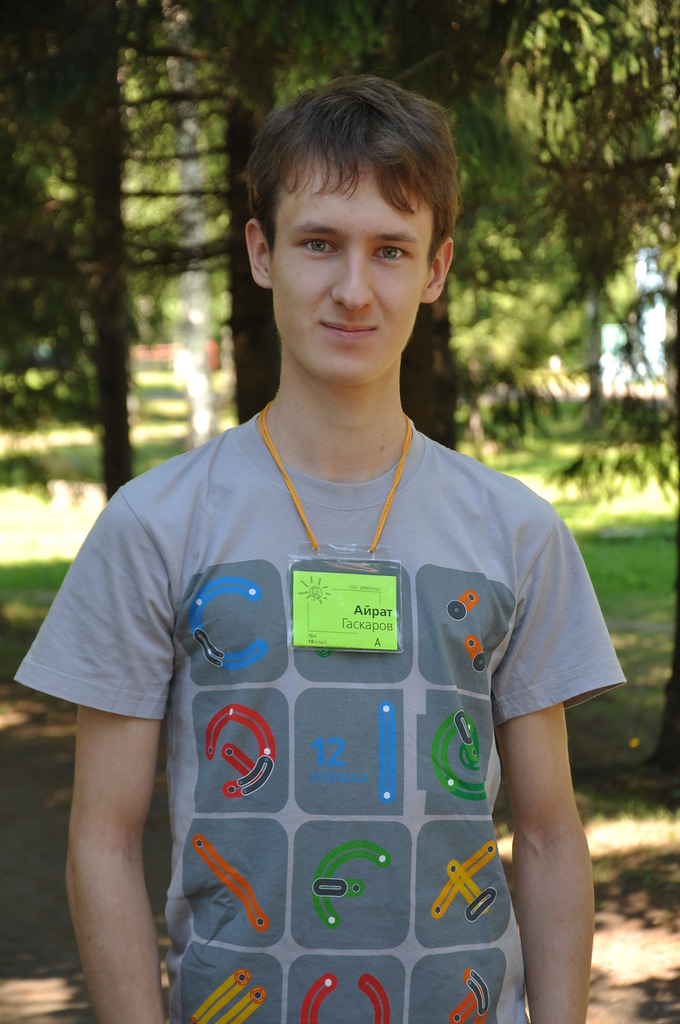
\includegraphics[width=0.5\linewidth]{../images/Airat.jpg}}
  \caption{Произвольная картинка}
\end{figure}

И мы хотим отделить фон от человека. То есть присвоить каждому пикселю матрицы
$n \times m$ какой-то label, к какому классу относится --- фон или человек,
например.

Фактически это единственный алгоритм машинного обучения, где используются
алгоритмы на потоках.

\textit{Прим. Те, кто не помнят, что такое поток, могут закрывать эту лекцию.}

\subsection{Минимизация парно-сепарабельной энергии от бинарных переменных}

Пусть у нас задан неориентированный граф $G(V, E)$. Для каждого $i \in V$ пусть
$x_i$ могут принимать значения только из $\{0, 1\}$.

\begin{Def}
  Назовём \textbf{энергией} (обозначение $I$) функцию из $\{0, 1\}^{|V|} \to
  \R$:
  \[
    I(X) = \sum_{i \in V} \theta_i(x_i) + \sum_{(i, j) \in E} \theta_{ij}(x_i, x_j) +
    \theta_0,
  \]

  где $\theta_i, \theta_{ij}$ --- какие-то потенциалы, а $\theta_0$ --- константа.
\end{Def}

И наша задача заключается в том, что минимизировать $I(X)$. Известно, что если
не вводить никаких дополнительных ограничений, то задача минимизации 
энергии является NP-трудной.

Давайте поймём, как
это относится к сегментации. На выборке из огромного числа изображений мы
можем с уверенностью говорить, о том, какие пиксели находятся рядом, какие
далеко по цвету, поэтому можем поставить какие-то веса на рёбрах. После этого
сегментировать изображение, чтобы были в одной и другой части как можно
более тёплые цвета. Рассмотрим частный случай потенциалов, в котором задача
становится полиномиальной:

\begin{itemize}
  \item $\forall \ i \in V, \theta_i(0) \geqslant 0, \theta_i(1) \geqslant 0$;
  \item $\forall \ (i, j) \in E \Rightarrow \theta_{ij}(0, 0) = \theta_{ij}(1, 1) = 0, 
  \theta_{ij}(0, 1) \geqslant 0, \theta_{ij}(1, 0) \geqslant 0$.
\end{itemize}

Тогда энергию можно задать так (легко проверить все случаи):

\[
  I(X) = \sum_{i \in V} (x_i\theta_i(1) + (1 - x_i)\theta_i(0)) + 
  \sum_{(i, j) \in E} (x_i(1 - x_j)\theta_{ij}(1, 0) + 
  x_j(1 - x_i)\theta_{ij}(0, 1)) + \theta_0,
\]

\begin{figure}[H]
  \center{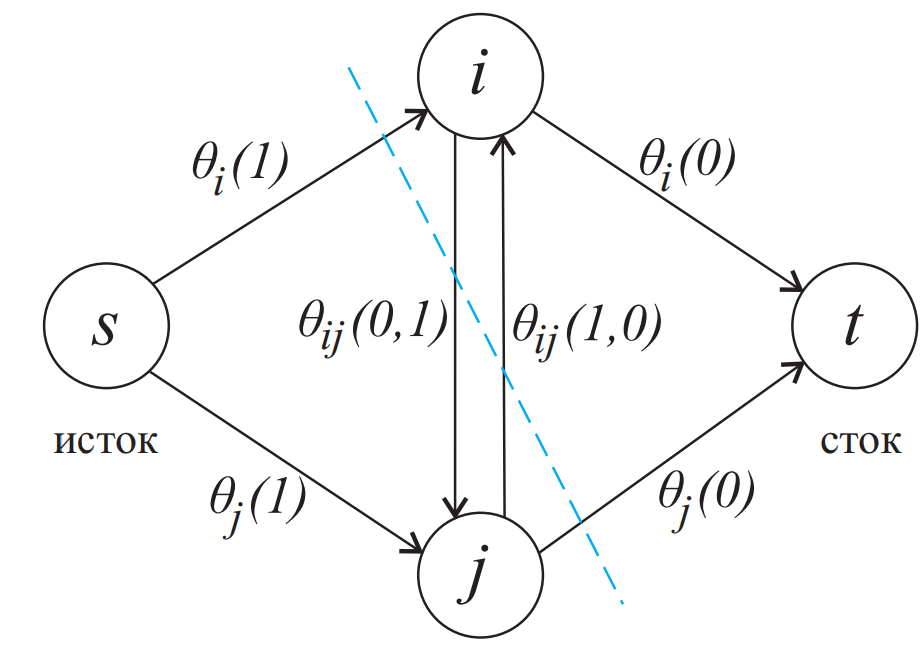
\includegraphics[width=0.5\linewidth]{../images/graph.png}}
  \caption{Граф, построенный для минимизации энергии от двух переменных
  $x_i, x_j$. Разрез, отображенной пунктирной линией соответствует присваиванию 
  $x_i = 1, x_j = 0$. Величина разреза составляет $\theta_i(1) + \theta_j(0) +
  \theta_{ij}(1, 0)$}.
\end{figure}

Теперь построим ориентированный граф $\overline{G} = (\overline{V}, \overline{E})$
по следующим правилам:

\begin{itemize}
  \item В $\overline{V} = V \cup \{s, t\}$;
  \item Неориентированные рёбра делаем ориентированными в обе
  стороны, а для каждой вершины
  $i$ проведем ещё ребра $(s, i), (i, t)$;
  \item $c(s, i) = \theta_i(1), c(i, t) = \theta_i(0)$, где $i \in V$;
  \item $\forall \ (i, j) \in E$ таким, что $i < j$ положим $c(i, j) =\theta_{ij}(0, 1), c(j, i) = \theta_{ij}(1, 0)$;
  \item Все вершины из $V$, которые попали в минимальный разрез $S$ положим $x_i = 0$,
  остальным $x_i = 1$.
\end{itemize}

Тогда видно, что минимизация разреза эквивалентна этой задаче, что эквивалентно
задаче максимального потока. Существует, конечно, много алгоритмов максимального
потока, многие из них мы изучали, но в компьютерном зрении часто возникают алгоритмы
Бойкова-Колмогорова и IBFS. С ними вы можете ознакомиться при желании самостоятельно.

Пример графа, построенного для энергии от 2-х переменных, и его разреза 
приведен на рис 2.

\subsection{Репараметризация}

Здесь мы рассмотрим, какие ещё энергии можно минимизировать при помощи
разрезов графов. Назовём преобразования потенциалов, не меняющее энергию 
\textit{репараметризацией}. Рассмотрим несколько видов репараметризаций:

\begin{itemize}
  \item Вычитание константы --- $\theta_i(0) \mathrel{{-}{=}} \delta, \theta_i(1) \mathrel{{-}{=}} \delta,
  \theta_0 \mathrel{{+}{=}} \delta$;
  \item Изменение потенциалов на ребрах. $\theta_{ij}(p, 0) \mathrel{{-}{=}} \delta, 
  \theta_{ij}(p, 1) \mathrel{{-}{=}} \delta, \theta_i(p) \mathrel{{+}{=}} \delta$. Аналогично, если
  $p$ на 2-ой координате.
\end{itemize}

Легко видеть из определения, что эти преобразования не меняют энергию.

Рассмотрим, что можно делать при помощи репараметризации потенциалов на ребрах.
Для $(i, j) \in E$ пусть 
$\theta_{ij}(0, 0) = a$,
$\theta_{ij}(1, 1) = b$,
$\theta_{ij}(0, 1) = c$,
$\theta_{ij}(1, 0) = d$.

После этого давайте 3 раза применим 2-ой пункт видов репараметризации:

\begin{itemize}
  \item $\theta_{ij}(0, 0) \mathrel{{-}{=}} a, \theta_{ij}(0, 1) \mathrel{{-}{=}} a, \theta_{i}(0) \mathrel{{+}{=}} a$;
  \item $\theta_{ij}(0, 1) \mathrel{{-}{=}} (c - a), \theta_{ij}(1, 1) \mathrel{{-}{=}} (c - a),
  \theta_{j}(1) \mathrel{{+}{=}} c - a$;
  \item $\theta_{ij}(1, 1) \mathrel{{-}{=}} (b - c + a), \theta_{ij}(1, 0) \mathrel{{-}{=}} (b - c + a),
  \theta_{i}(1) \mathrel{{+}{=}} b - c + a$
\end{itemize}

Потом сделаем все потенциалы вершины неотрицательными по 1-ому пункту
репараметризации. В итоге у нас ненулевым останется только $\theta_{ij}(1, 0) =
d + c - a - b$. И если оно положительно, то мы можем применить наш алгоритм, то
есть должно выполняться условие \textit{субмодулярности}:

\[
  \theta_{ij}(0, 0) + \theta_{ij}(1, 1) \leqslant \theta_{ij}(0, 1) + 
  \theta_{ij}(1, 0)
\]

Данное условие вызвано тем, что для полиномиальной разрешимости задач о 
максимальном потоке и минимальном разрезе пропускные способности дуг графа
должны быть неотрицательны.

\subsection{$\alpha$-расширение}

Мы умели решать задачу только с одним объектом, теперь давайте попробуем
приближенно решить задачу со многими объектами. Тот же граф, только теперь
поставим в соответствие каждой вершине $i$ --- $y_i \in \{1, \ldots, K\}$ ---
классы разбиения. Рассмотрим следующую энергию:

\[
  I_M(X) = \sum_{i \in V} \psi_i(x_i) + \sum_{(i, j) \in E} \psi_{ij}(x_i, x_j) +
    \psi_0,
\]

Буква $M$, скорее всего, идёт от английского слова Many --- много.

Алгоритм $\alpha$-расширение минимизирует энергию при помощи выполнения шагов между 
разметками $y$, каждый из которых гарантированно не увеличивает значение энергии. 
Каждый шаг
представляет собой задачу минимизации энергии бинарных переменных вида.
Неформально каждый шаг позволяет каждой переменной из $y$ либо присвоить выбранное значение 
$\alpha$, либо оставить текущее значение (расширение метки $\alpha$).

\begin{figure}[H]
  \center{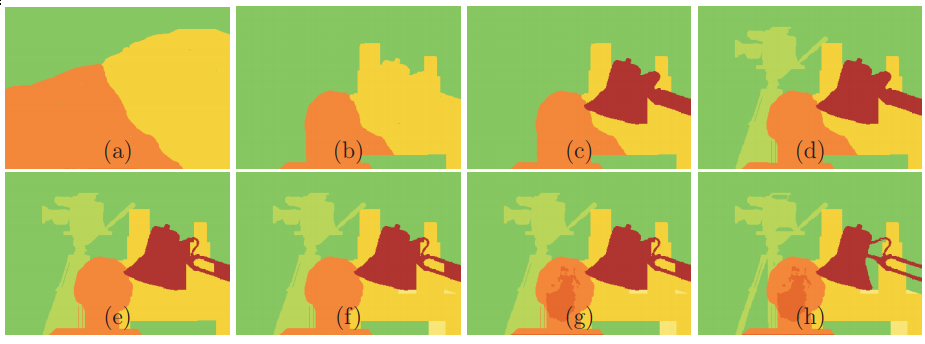
\includegraphics[width=1\linewidth]{../images/alpha.png}}
  \caption{Пример работы алгоритма $\alpha$-расширения для задачи
  выровненного стерео. (a) -- начальная разметка, далее последовательные
  расширения различных меток.}
\end{figure}

На каждом шаге алгоритма у нас есть текущее приближение $y^0$ и выбрана
\textit{расширяемая} метка $\alpha \in \{1, \ldots, K\}$.

\begin{itemize}
  \item Граф, потенциалы сначала одинаковы;
  \item Применяем алгоритм о минимальном разрезе, теперь, если $x_i = 0$, то
  остовляем $y_i^0$, а если $x_i = 1$, то меняем переменную $y_i^0 = \alpha$;
  \item Меняем все потенциалы вершин: $\theta_i(0) = \psi_i(y_i^0), 
  \theta_i(1) = \psi_i(\alpha);$
  \item Меняем потенциалы на ребрах: $\theta_{ij}(0, 0) = \psi_{ij}(y_i^0, y_j^0),
  \theta_{ij}(1, 1) = \psi_{ij}(\alpha, \alpha), \theta_{ij}(0, 1) =
  \psi_{ij}(y_i^0, \alpha), \\\theta_{ij}(1, 0) = \psi_{ij}(\alpha, y_j^0)$;
  \item Повторяем процедуру, сколько нам надо для реальной задачи.
\end{itemize}

\end{document}

\oball
\newpage
\documentclass[a4paper, 12pt]{article}
\usepackage{header}

\begin{document}
\pagestyle{fancy}

\section{$\Pclass$ vs. $\NPclass$}

\subsection{Класс $\Pclass$ и сведение}

Сейчас мы переходим в теоретический материал, который является основой
классификации алгоритмов. Нас совершенно не интересует эффективность, кроме
как разделение на <<алгоритмы, которые работают за полиномиальное время>> и все
остальные.

Договоримся, что мы определяем <<алгоритм>>, как детерминированную
машину Тьюринга. И будем
использовать тезис Чёрча-Тьюринга о том, что любая вычислимая функция является
вычислимой на машине Тьюринга. Также условимся, что мы рассматриваем только
задачи принятия решения (принадлежит ли слово)

\begin{Def}
  Задача $A \in \Pclass$ (формально говоря язык), если существует машина Тьюринга,
  проверяющая принадлежность
  слова языку,
  время работы $t_A(x)$ которой ограничено полиномом от $P(|x|)$, который является
  фиксированным для всех входов.
\end{Def}

Также, до определения класса $\NPclass$, определим,
что значит язык $A$ сводится к языку $B$ за полиномиальное время.

\begin{Def}
    Язык $A$ \textbf{сводится} к языку $B$ за полиномиальное время, если 
    существует функция $f$, вычислимая за полиномиальное время, такая, что 
    $w \in A \Longleftrightarrow f(w) \in B$.
    Обозначение: $A \leqslant_p B$.
\end{Def}
Докажем основное утверждение о сводимости:
\begin{Statement}
    Пусть $A \leqslant_p B$ и $B \in \Pclass$ (существует полиномиальный 
    алгоритм решения задачи). Тогда $A \in \Pclass$.
\end{Statement}

\begin{proof}
 Достаточно построить алгоритм, показывающий, что для языка $A$ тоже существует 
 полиномиальное решение. Пусть у нас имеются МТ $M_A$, допускающая язык $A$, и 
 $M_B$, допускающая язык $B$. Поскольку $A \leqslant_p B$, то $\exists$ 
 полиномиальная $f$, удовлетворяющая определению выше. Построим алгоритм вычисления $M_A$:
 \begin{algorithmic}
    \Require{слово $w$}
    \State вычислить $f(w)$
    \State \Return $M_B\big(f(w)\big)$
 \end{algorithmic}
 Поскольку сама функция $f$ является вычислимой за полиномиальное время, то 
 вычисление $f(w)$ потратит полиномиальное время. Кроме того, поскольку 
 $B \in \Pclass$, то вычисление $M_B\big(f(w)\big)$ также займёт полиномиальное 
 время (от размера $f(w)$, но $f(w)$ также вычисляется за полином)! Отсюда 
 $M_A(w)$ также допускает слово $w$ за полиномальное время, что по определению 
 означает, что $A \in \Pclass$.
\end{proof}

\subsection{$\NPclass$ класс}

\begin{Def}
  Язык \(L\) лежит в классе \(\NPclass\), если существует функция 
  от двух аргументов \(A(x, y)\)~--- \textbf{алгоритм верификации}~---  с 
  полиномиальной сложностью от \(x\) такая, что \(x\) лежит в \(L\) 
  тогда и только тогда, когда для него существует \(y\) (его принято называть 
  \textbf{сертификатом}) такой, что \(A(x, y) = 1\). При этом сертификат должен
  быть полиномиально зависим от размера \(x\).
\end{Def}

Ясно, что $\Pclass \subseteq \NPclass$, так как за алгоритм верификации можно
взять просто полиномиальный алгоритм принадлежности слова языку.

Также введём понятие $\coNPclass$ класса:

\begin{Def}
  \[
    \coNPclass = \{\overline{L} = \Sigma^{*} \setminus L \mid L \in \NPclass\}
  \]
\end{Def}

Другими словами, $\coNPclass$~--- множество всех языков, которые могут
верифицировать \textbf{не}принадлежность слово языку. Например, такая задача
--- <<Нет ли гамильтонового цикла в графе?>>. Неизвестно, лежит ли она в $\NPclass$,
но она точно лежит в $\coNPclass$ (оставляем упражнение читателю, как предъявить
верификатор). Также ясно, что $\Pclass \subseteq \coNPclass$.

Оставим тоже следующую лемму, как упражнение читателю (думаем, что 2 определения
должны быть интуитивно понятны):

\begin{Lemma}
  $\NPclass \subseteq \mathsf{PSPACE} \subseteq \mathsf{EXPTIME}$ 
\end{Lemma}

\subsection{$\NPCclass$ классы и теорема Кука-Левина}

\begin{Def}
  Язык $A$--- $\NPclass$-трудный, если $\forall \ B \in \NPclass : B \leqslant_p A$.
\end{Def}

\begin{Def}
  Язык $A \in \NPCclass$ ($\NPclass$-complete или Nondeterministic Polynomial 
  Complete), если $A \in \NPclass$ и $\forall \ B \in \NPclass \implies B
  \leqslant_p A$.
\end{Def}

Другими словами, $\NPCclass$~--- это в точности те языки, которые являются
сами $\NPclass$ и $\NPclass$-трудными одновременно.

Докажем следующие простые утверждения:

\begin{Lemma}
  Пусть $L \in \NPCclass$. Тогда, если $L \in \Pclass$, то $\Pclass = \NPclass$.
\end{Lemma}
\begin{proof}
  Пусть $L' \in \NPclass$. Так как $L \in \NPCclass$, то $L' \leqslant_p L$.
  Но, поскольку $L \in \Pclass$, то $L' \in \Pclass$, откуда $\Pclass = \NPclass$.
\end{proof}

\begin{Lemma}
Если $B \in \NPCclass$ и $B \leqslant_p C \in \NPclass$, то $C \in \NPCclass$.
\end{Lemma}
\begin{proof}
  Проверим оба условия, входящих в определение $\NPclass$-полного класса.
  \begin{enumerate}
    \item $C \in \NPclass$ -- по условию.
    \item Пусть $L' \in \NPclass$. Так как $B \in \NPCclass$, то $L' 
    \leqslant_p B$, что по определению означает, что существует некая 
    функция $f_{L'B}$
    (которая сводит одну задачу к другой), вычислимая за полиномиальное 
    время. Кроме того, $B \leqslant_p C$, что по определению означает, что 
    существует некая функция $f_{BC}$, вычислимая за полиномиальное время.
        
    Но это означает, что $L' \leqslant_p C$, так как существует функция 
    $f_{L'C}$, такая, что $f_{L'C}(w) = f_{BC}\big(f_{L'B}(w)\big)$ -- она 
    также является вычислимой за полиномиальное время.
        
    Следовательно, $\forall\ L' \in \NPclass: L' \leqslant_p C$, откуда 
    $C$ -- $\NPclass$-трудный по определению.
  \end{enumerate}
  Оба условия выполняются, значит, $C \in \NPCclass$.
\end{proof}

Но всё равно должны же остаться вопросы по тому, зачем всё это надо и как
вообще доказывать, что задача трудна, то есть лежит в классе $\NPclass$. 
Ведь должна же быть какая-то <<первая>> задача из $\NPCclass$. Если вы решаете
задачу и вдруг понимаете, что она эквивалентна какой-то задаче из $\NPCclass$,
то возможно стоит либо перечитать задачу (и понять, каким условием
надо точно пользоваться), либо решить и получить $\$1\,000\,000$.

Одна из первых $\NPCclass$ задач была задача $SAT$ (от англ.
Satisfiability). Можем считать, что нам
дана булева формула в конъюнктивно нормальной форме. Сейчас мы покажем, что
любая $\NPclass$ задача сводится к этой. Вообще, так как если мы хотим сводить
любую $\NPclass$ задачу к $SAT$, то какие-то обычные рассуждения вряд ли пройдут.
Действительно, мы будем стараться моделировать работу МТ через КНФ.

\begin{Theorem}[Теорема Кука-Левина]
  $SAT \in \NPCclass$.
\end{Theorem}

\begin{proof}
  Сначала покажем, что $SAT \in \NPclass$. Действительно, по входу булевой
  формулы и верификатору (значение переменных $x_1, \ldots, x_n$) мы с лёгкостью
  проверим выполнимость формулы. Поэтому есть линейный алгоритм верификации.

  Пусть $\mathcal{P} \in \NPclass$. Надо понять, как полиномиально свести
  эту задачу к $SAT$. По определению класса $\NPclass$ существует полином
  $p$ и алгоритм $\mathcal{P'}$, который верифицирует задачу $\mathcal{P}$, 
  причём верификатор размера не больше, чем $|p(|x|)|$.

  Пусть
  \[
    \Phi : \{0, \ldots, N\} \times \overline{A} \to \{-1, \ldots, N\}
    \times \overline{A} \times \{-1, 0, 1\}
  \]
  МТ, работающая за полиномиальное время, отвечающая за задачу $\mathcal{P'}$
  с алфавитом $A$. Добавим пустой символ к $A$, чтобы легче было работать.
  Пусть работа этой МТ ограничена полиномом $q$, то есть time$(\Phi, x\#c)
  \leqslant q(|x\#c|)$. Сейчас мы соорудим набор дизъюнктов 
  (или клауз) $Z(x)$, который
  ограничен полиномом $Q \gets q(|x\#c|)$, такой, что $Z(x)$ выполняется
  тогда и только тогда, когда слово принадлежит языку $\mathcal{P}$.

  Ясно, что мы не уйдём за пределы ленты от $-Q$ до $Q$.

  Теперь создадим несколько переменных:
  \begin{itemize}
    \item переменные $v_{ij\sigma}$ для всех $0 \leqslant i \leqslant Q$,
    $-Q \leqslant j \leqslant Q$ и $\sigma \in \overline{A}$. Верно ли, что
    в момент $i$ (после $i$ шагов выполнения МТ) позиция с номером $j$ содержала
    символ $\sigma$.

    \item переменные $w_{ijn}$ для всех $0 \leqslant i \leqslant Q$,
    $-Q \leqslant j \leqslant Q$ и $-1 \leqslant n \leqslant N$. Верно ли, что
    в момент $i$ на позиции $j$ МТ была в состоянии $n$. За минус 1 отвечает
    финальное состояние.
  \end{itemize}

  Поэтому, если у нас есть конфигурация МТ на $i$-ом шаге
  с позицией $\pi^{(i)}$, символами $s^{(i)}$ и состоянием $n^{(i)}$, тогда
  мы должны выставить $v_{ij\sigma} := true$ тогда и только тогда, когда
  $s_j^{(i)} = \sigma$ ($s_j$ --- позиция на $j$-ом месте ленты МТ). И мы должны
  выставить $w_{ijn} := true$ тоже тогда и только тогда, когда $\pi^{(i)} = j$ и
  $n^{(i)} = n$.

  Сейчас мы предъявим набор клауз $Z(x)$, который будет выполняться тогда и
  только тогда, когда существует строка $c$ полиномиального размера, что 
  МТ $\Phi$ на входе $x\#c$ выдаёт единицу.

  В каждый момент времени на каждой позиции стоит строго один символ:

  \begin{itemize}
    \item дизъюнкт $(v_{ij\sigma} \mid \sigma \in \overline{A})$ по всем 
    $0 \leqslant i \leqslant Q$ и $-Q \leqslant j \leqslant Q$.
    \item $(\overline{v_{ij\sigma}}, \overline{v_{ij\tau}})$ по всем 
    $0 \leqslant i \leqslant Q$, и $-Q \leqslant j \leqslant Q$, и $\sigma \neq
    \tau \in \overline{A}$.
  \end{itemize}

  В каждый момент времени единственная позиция в строке сканируется и
  единственная инструкция выполняется:

  \begin{itemize}
    \item $(w_{ijn} \mid -Q \leqslant j \leqslant Q, -1 \leqslant n \leqslant N)$
    для всех $0 \leqslant i \leqslant Q$.
    \item $(\overline{w_{ijn}}, \overline{w_{ij'n'}})$ по всем 
    $0 \leqslant i \leqslant Q$ и $-Q \leqslant j, j' \leqslant Q$ и 
    $-1\leqslant n, n' \leqslant N$ с условием, что $(j, n) \neq (j', n')$.
  \end{itemize}

  Алгоритм корректно начинает свою работу:

  \begin{itemize}
    \item $(v_{0, j, x_j})$ по всем $1 \leqslant j \leqslant |x|$.
    \item $(v_{0, |x| + 1, \#})$ --- разделяющий символ.
    \item $(v_{0, |x |+ 1 + j, 0}, v_{0, |x| + 1 + j, 1})$
    по всем $1 \leqslant j \leqslant p(|x|)$.
    \item $(v_{0, j, \sqcup})$ по всем $-Q \leqslant j \leqslant 0$ и
    $|x| + 2 + p(|x|) \leqslant j \leqslant Q$ --- пустые символы не с входа.
    \item $(w_{0,1,0})$ --- начальное положение головки.
  \end{itemize}

  Алгоритм работает корректно:

  \begin{itemize}
    \item $(\overline{v_{ij\sigma}}, \overline{w_{ijn}}, v_{i + 1, j, \tau})$ и
    $(\overline{v_{ij\sigma}}, \overline{w_{ijn}}, w_{i + 1, j + \delta, m})$
    по всем $0 \leqslant i < Q, -Q \leqslant j\leqslant Q; \sigma, \tau \in 
    \overline{A}, \delta \in \{-1, 0, 1\}$, где $\Phi(n, \sigma) = 
    (m, \tau, \delta)$ (переход по состоянию $n$, символу $\sigma$ в какое-то
    состояние $m$, символ $\tau$ пишем на $j$-ом месте и сдвиг на $-1, 0$ или $1$).
  \end{itemize}

  Когда алгоритм достигает финального состояния (минус 1 в нашем случае), алгоритм
  останавливается:
  \begin{itemize}
    \item $(\overline{w_{i, j, -1}}, w_{i + 1, j, -1})$ и 
    $(\overline{w_{i, j, -1}}, \overline{v_{i, j, \sigma}}, v_{i + 1, j, \sigma})$
    по всем $0 \leqslant i < Q; -Q \leqslant j \leqslant Q$ и $\sigma \in
    \overline{A}$ --- как раз, если достигли состояния $-1$, тогда все состояния
    в каждое время должны быть минус один и символ меняться не должен.
  \end{itemize}

  Позиции, которые не были просмотрены, должны остаться неизменными:

  \begin{itemize}
    \item $(\overline{v_{ij\sigma}}, \overline{w_{ij'n}}, v_{i+1, k, \sigma})$
    по всем $0 \leqslant i \leqslant Q; \sigma \in \overline{A}; -1 \leqslant
    n \leqslant N$ и $-Q \leqslant j, j' \leqslant Q$ при условии, что $j \neq j'$.
  \end{itemize}

  Алгоритм выводит единицу:
  \begin{itemize}
    \item $(v_{Q, 1, 1})$ и $(v_{Q, 2, \sqcup})$ --- на первой позиции стоит
    единица, а потом пробел (можно считать, что только один, можно, что все
    последующие, это не играет на роль полиномиальности МТ и полиномиальности
    размера КНФ).
  \end{itemize}

  Заметим, что размер $Z(x)$ будет не больше, чем $\O(Q^3\log Q)$, существует
  $\O(Q^3)$ литералов и нужно $\O(\log Q)$ памяти, чтобы закодировать индексы.

  Осталось показать, что $Z(x)$ выполняется тогда только тогда, когда $x$
  принадлежит языку.

  Если $Z(x)$ выполняется, то пусть $T$ --- это набор переменных, удовлетворяющим
  всем клаузам. Поставим $c_j = 1$ по всем $j$ для которых 
  $T(v_{o, |x| + 1 + j, 1}) = true$ и $c_j = 0$ в ином случае. Сверху мы
  описали работу МТ $\Phi$ на входе $x\#c$. Поэтому мы можем заключить, что
  $\Phi(x\#c) = 1$. Так как $\Phi$ --- алгоритм верификации, то это значит, что
  $x$ принадлежит языку.

  Пусть $x$ принадлежит языку. Тогда пусть $c$ --- сертификат проверки для $x$.
  Тогда пусть конфигурация МТ на входе $x\#c$ на $i$-ом шаге пусть будет равна 
  $(n^{(i)}, s^{(i)}, \pi^{(i)})$. Тогда давайте поставим $T(v_{i,j,\sigma}) = 
  true$ тогда и только тогда, когда $s_j^{(i)} = \sigma$ и $T(w_{i, j, n})=true$
  тогда и только тогда, когда $\pi^{(i)} = j, n^{(i)} = n$ по всем $i \leqslant m$.
  Для б\'{о}льших $i$ выставим $T(v_{i, j, \sigma}) := T(v_{i - 1, j, \sigma})$
  и $T(w_{i, j, n}) := T(w_{i - 1, j, n})$ по всевозможным $j, n, \sigma$. Тогда
  можно убедиться, что формула выполняется, что завершает наше доказательство.
\end{proof}


\end{document}

\oball
\newpage
\documentclass[a4paper, 12pt]{article}
\usepackage{header}

\begin{document}
\pagestyle{fancy}

\section{$\NPclass$ классы, сведения, различные другие классы алгоритмов}

\epigraph{<<Будет вообще уморительно, если кто-то сядет и скажет: <<Ох ё,
поиск Гамильтонова цикла это просто динамика за квадрат>>. И полстраницы кода...>>}
{Глеб}

В прошлый раз мы поговорили о просто задаче $SAT$. Теперь у нас есть мощный
инструмент к сведению сложных на данное время задач. Первая из них ---
3-$SAT$ --- булева формула в конъюктивно нормальной форме, где каждый дизъюнкт
содержит не более 3 литералов (ну или ровно 3, мы докажем эквивалентность чуть
позже).

\subsection{Сведение $SAT$ к 3-$SAT$}

\begin{Theorem}
  $SAT \leqslant_p$ 3-$SAT$.
\end{Theorem}

\begin{proof}
  Возьмём один дизъюнкт и сделаем из него много дизъюнктов с количеством
  литералов не более 3.

  Действительно, пусть у нас будет дизъюнкт $(x_1 \vee \ldots \vee x_{k})$ --- 
  возможно
  с отрицаниями, нам не важно. Разобьём на 2 примерно равных множества этот
  дизъюнкт --- в одном $\left\lfloor \frac{k}{2} \right\rfloor$ литералов, в
  другом $\left\lceil \frac{k}{2} \right\rceil$. Добавим новую переменную $x_{n + 1}$,
  тогда покажем эквивалентность $(x_1 \vee \ldots \vee 
  x_{\lfloor k/2\rfloor} \vee x_{n + 1}) \wedge (x_{\lfloor k/2 \rfloor + 1}
  \vee \ldots \vee 
  x_{k} \vee \overline{x_{n + 1}})$. Действительно, если эти 2 дизъюнкта выполнены,
  то в одном из них литерал с $x_{n + 1}$ равен 0, значит один из литералов
  в множестве $x_1, \ldots, x_k$ равен 1 и изначальный дизъюнкт выполнен.

  В другую сторону --- если изначальный дизъюнкт выполнен, тогда существует
  какой-то литерал из $x_1, \ldots, x_k$, который равен 1, тогда поставим $x_{n + 1}$
  так, что оно равно 0, там где литерал из $x_1, \ldots, x_k$ равен 1. Тогда
  обе скобки будут равны единице (там, где есть литерал, который равен 1, будет
  всегда 1, а в другой скобке литерал с $x_{n + 1}$ равен 1).

  Будем так делать для каждого дизъюнкта, добавляя новую (обязательно не
  совпадающую с предыдущими созданными) переменными. И будем останавливаться,
  когда дизъюнкт содержит не более 3 литералов. Заметим, что из дизъюнкта,
  состоящего из 3 литералов нельзя сделать 2 дизъюнкта со строго меньшим
  количеством литералов. Легко проверить, что такая процедура работает только
  при $k \geqslant 4$. 

  Осталось совсем немного --- доказать, что 3-$SAT \in \NPclass$ и сведение
  действительно полиномиально. Первое совсем очевидно, так как 3-$SAT$ это
  частный случай $SAT$, а про $SAT$ мы точно знаем, что эта задача из класса
  $\NPclass$.

  Заметим, что количество уровней при процедуре с одним дизъюнктом будет не более,
  чем $O(\log n)$ (это легко показать, сказав и проверив, что если проделать
  2 уровня, то максимальная длина дизъюнкта уменьшается хотя бы в 2 раза). И на
  каждом уровне мы создаём не более $2^k$ новых литералов. Если всё просуммировать,
  получим линейное сведение одного дизъюнкта. Для осталальных проделаем то же
  самое.
\end{proof}

Также стоит отметить по лемме в прошлой лекции следует, что 3-$SAT \in \NPCclass$.

Пока никто не умеет сводить $SAT$ к 2-$SAT$, так как последняя решается за
линейное время.

{\bf Байка от Глебаса:} Только испанские составители контестов могут 
это делать. Писали испанский контест. 
Читаешь условие --- вот просто дана задача о рюкзаке. 
$n \leqslant 50000,  a_i \leqslant 10^9$, TL 2 секунды.
Зашли в админку, увидели супер-эвристику, долго ржали, возможно, даже отослали 
решение, но не помню. Ну также они дали задачу на гамильтонов путь на 200 вершинах.

\subsection{$\NPclass$-полнота задач клики, доминирующего множества и вершинного
покрытия}

Ну теперь мы займёмся сведениями. Мы много говорили, что некоторые задачи на
графах очень сложны. Теперь надо ответить за базар:

\begin{Theorem}
  Задача <<существует ли клика размера $k$ в графе $G(V, E)$>> является $\NPCclass$.
\end{Theorem}

\begin{proof}
  Сведем эту задачу к $SAT$ (просто красивое рассуждение).
  Потом сделаем в другую сторону.

  \begin{center}
    \begin{tikzpicture}
      \tikzstyle{main node}=[draw,circle,fill=white,minimum size=4pt,
                            inner sep=0pt]
      \tikzstyle{every node}=[fill=white,minimum size=0pt]
      \draw (0, 0) node[main node](x_1) [label=left:$x_1$] {};
      \draw (5, 2) node[main node](x_2) [label=above:$x_2$] {};
      \draw (7, 2) node[main node](x_3) [label=above:$x_3$] {};
      \draw (10, 0) node[main node](x_4) [label=right:$x_4$] {};
      \draw (4.5, -3) node[main node](x_{n - 1}) [label=below:$x_{n - 1}$] {};
      % \draw (7, -1) node[main node](x_t1) [label=right:] {};
      % \draw (6.5, -1.5) node[main node](x_t12) [label=right:] {};
      % \draw (6, -2) node[main node](x_t13) [label=right:] {};
      \draw (1, -3) node[main node](x_n) [label=below:$x_n$] {};
      \node at ($(x_4)!.5!(x_{n - 1})$) {\huge{\reflectbox{$\ddots$}}};

      \draw (x_3) -- (x_n);
      \draw (x_1) -- (x_{n - 1});
      \draw (x_4) -- (x_n);
      \draw (x_2) -- (x_{n - 1});
      \draw (x_2) -- (x_4);
    \end{tikzpicture}
  \end{center}

  Переменные будут отвечать за вершины. Соорудим нашу формулу:

  Любые 2 вершины, между которыми нет ребра, не могут быть взяты обе.
  \begin{itemize}
    \item $(\overline{x_v}, \overline{x_u})$ при всех $(v, u) \not\in E$.
  \end{itemize}

  Введём такую величину --- $d_{ij}$, отвечающую на вопрос, верно ли, что
  среди первых $i$ вершин есть клика размера $j$. Заметим, что 
  $d_{ij} = d_{i - 1, j} \vee (d_{i-1,j-1} \wedge x_i)$, то есть либо есть
  клика размера $k$ среди первых $i - 1$ вершины, либо среди первых $i - 1$
  есть клика размера $j - 1$ и взята вершина $i$.

  \begin{itemize}
    \item $(\overline{d_{ij}} \vee d_{i - 1, j} \vee d_{i - 1, j - 1}) \wedge
    (\overline{d_{ij}} \vee d_{i - 1, j} \vee x_i)$ --- если $d_{i - 1, j} = 0$
    и $x_i = 0$, тогда точно $d_{ij} = 0$ и выполняются оба дизъюнкта.
    Если $d_{i - 1, j} = 0$ и $d_{i - 1, j - 1} = 0$, то $d_{ij} = 0$ в обоих
    случаях. Это делаем при $1 \leqslant i \leqslant n; 1 \leqslant j \leqslant k$.

    \item $(d_{ij} \vee \overline{d_{i - 1, j}}) \wedge (d_{ij}
    \vee \overline{d_{i - 1, j - 1}} \vee \overline{x_i})$. Это те же условия,
    только мы здесь хотим сделать $d_{ij} = 1$, если выполнено хотя бы одно
    условие. Это делаем при $1 \leqslant i \leqslant n; 1 \leqslant j \leqslant k$.
  \end{itemize}

  Начальные условия (среди первых ):

  \begin{itemize}
    \item $d_{0j} = 0$ при $1 \leqslant j \leqslant k$ --- среди нуля вершин
    нет клики размера хотя бы 1.
    \item $d_{i0} = 1$ при $0 \leqslant i \leqslant n$ --- среди первых
    $i$ вершин есть клика размера 0.
  \end{itemize}

  Финальное состояние:

  \begin{itemize}
    \item $(d_{nk})$ --- ответ на задачу.
  \end{itemize}

  Легко видеть, что это и есть $SAT$, притом формула выполняется тогда и только
  тогда, когда есть клика размера $k$. Причём сведение, очевидно, полиномиально.

  Теперь в другую сторону:

  Рассмотрим любую $SAT$ формулу. Пусть у нас есть $k$ дизъюнктов.
  Выпишем всех их (каждый литерал --- отдельная вершина) в виде графа.
  Внутри дизъюнкта вершины не будем соединять,
  а также не будем соединять вершины в различных дизъюнктах, которые отвечают
  сразу за $x_i$ и $\overline{x_i}$. Теперь запустим решение задачи о поиске
  клики размера $k$. Если решение нашлось, то в каждой части графа, отвечающего
  за отдельный <<дизъюнкт>>, выбрана ровно 1 вершина. Иначе в каком-то дизъюнкте
  выбрано 2, а мы не соединяли вершины в одном и том же дизъюнкте. Поэтому
  в каждом дизъюнкте выбран ровно 1 литерал. Сделаем эти литералы равными единице.
  Те переменные, которые мы не выбрали, положим единице. Заметим, что мы
  не сделали одновременно $x_i$ и $\overline{x_i}$ равными единице, так как
  иначе между ними было бы ребро. А мы договорились, что такого ребра нет.

  То, что любому решению $SAT$ формулы соответствует какая-то клика в построенном
  графе следует из почти дословных рассуждений выше, что завершает док-во, что
  задача про поиск клики данного размера лежит в $\NPCclass$.
\end{proof}

Теперь поговорим про задачу о доминирующем множестве размера $k$. Напомним, что мы
хотим в данной задаче найти $k$ вершин так, что оставшиеся вершины соединены
хотя бы с одной из выбранных вершин. Докажем следующее сведение:

\begin{Theorem}
  $Dominant\_set \in \NPCclass$.
\end{Theorem}

\begin{proof}
  Сведём $SAT$ к этой задаче.

  Пусть $f_1, \ldots, f_k$ --- дизъюнкты в формуле $SAT$. Тогда построим следующий
  граф:

  \begin{center}
    \begin{tikzpicture}
      \tikzstyle{main node}=[draw,circle,fill=white,minimum size=4pt,
                            inner sep=0pt]
      \tikzstyle{every node}=[fill=white,minimum size=0pt]
      \draw (0, 0) node[main node](x_1) [label=left:$x_1$] {};
      \draw (1, 0) node[main node](nx_1) [label=above:$\overline{x_1}$] {};

      \draw (2, 0) node[main node](x_2) [label=above:$x_2$] {};
      \draw (3, 0) node[main node](nx_2) [label=above:$\overline{x_2}$] {};

      \draw (5, 0) node[main node](x_n) [label=above:$x_{n}$] {};
      \draw (6, 0) node[main node](nx_n) [label=above:$\overline{x_{n}}$] {};

      % \draw (1, -3) node[main node](x_n) [label=below:$x_n$] {};
      \node at ($(x_2)!.65!(x_n)$) {$\ldots$};

      \draw (-1, -3) node[main node] (f_1) [label=below:$f_1$] {};
      \draw (1, -3) node[main node] (f_2) [label=below:$f_2$] {};
      \draw (5, -3) node[main node] (f_{t - 1}) [label=below:$f_{t - 1}$] {};
      \draw (7, -3) node[main node] (f_t) [label=below:$f_t$] {};
      \node at ($(f_2)!.5!(f_{t - 1})$) {$\ldots$};



      \draw (x_1) -- (nx_1);
      \draw (x_2) -- (nx_2);
      \draw (x_n) -- (nx_n);
      \draw (f_1) to [out=50,in=-50] (x_2);
      \draw (f_{t - 1}) to [out=50,in=-50] (nx_1);
      \draw (f_1) to [out=50,in=-50] (nx_1);
      \draw (f_2) to [out=-50,in=-50] (x_n);
      \draw (x_1) to [out=90,in=100] (f_t);

    \end{tikzpicture}
  \end{center}

  Соединим литералы с теми дизъюнктами, куда он входит, а также соединим
  рёбрами $x_i$ и $\overline{x_i}$.

  \textbf{Обязательно надо сделать $n + 1$ копию каждого $f_i$ и соединить их
  также, как я показал на графе.}

  Теперь докажем, что доминирующее множество размера $n$ в графе будет
  соответствовать решению и наоборот.

  Если есть решение булевой формулы в КНФ, то если $x_i = 1$, возьмём в
  доминирующее множество вершину $x_i$, иначе $\overline{x_i}$. Заметим, что
  если формула выполняется, то в каждом дизъюнкте хотя бы один литерал равен 1.
  Заметим, что мы его взяли в доминирующее множество. Также все $x_i, \overline{x_i}$
  будут покрыты какой-то вершиной, так как мы берем точно одно из двух.

  В обратную сторону. Пусть нам было сказано, что доминирующее множество размера
  $n$ существует. Заметим, что если при фиксированном $i$ ни одна вершина из 
  пары вершин $x_i, \overline{x_i}$ не взята в доминирующее множество, то в
  доминирующее множество взято какое-то из $f_k$ (пусть оно соединено с $x_i$). Все $f_k$ сразу быть взяты
  не могли (их $n + 1$), значит существует $f_k$, которое не взяли в доминирующее
  множество. Тогда существует $x_k$ или $\overline{x_k}$, которое соединено
  с этим <<не взятым>> $f_k$, а значит оно соединено со всеми $f_k$, значит мы
  можем не брать никакое $f_k$ в доминирующее множество, а взять $x_i$. Тогда
  не нарушится свойство доминирующего множества и элементов мы возьмём ровно $n$.
  Так можно избавиться от всех вершин в доминирующем множестве, которые являются
  вершинами $f_k$. Значит существует доминирующее множество на $n$ вершинах только
  из $x_i$ и $\overline{x_i}$. Если обе вершины при фиксированном $i$ взяты,
  то по принципу Дирихле существует пара $x_j, \overline{x_j}$, из которой
  не взяли ни одну вершину в доминирующее множество. А этот случай см. выше.

  Теперь тем литералам, которые мы взяли, поставим единицу. Ясно, что они
  друг другу не противоречат (см. выше) и каждый дизъюнкт будет выполнен, так
  как эти $n$ вершин образуют доминирующее множество, то есть каждый дизъюнкт
  соединен с какой-то вершиной из доминирующего множества.

  Понятно, что мы провели полиномиальное сведение от размера КНФ.

  Ясно, что по множеству вершин легко проверить, является ли оно доминирующим
  (например, если взять матрицу смежности и проверить каждую вершину за полином).
  Поэтому мы свели $\NPCclass$ задачу к этой, а эта задача оказалась из $\NPclass$,
  значит эта задача является $\NPclass$-трудной.
\end{proof}

Теперь поговорим о вершинном покрытии графа размера $k$. 
Вспомним, что вершинное покрытие
это множество вершин такое, что любое ребро инцидентное хотя бы одной вершине
из множества. Неудивительно, эта задача тоже $\NPCclass$.

\begin{Theorem}
  $Vertex\_cover \in \NPCclass$.
\end{Theorem}

\begin{proof}
  Сведём 3-$SAT$ к этой задаче.

  Ну здесь как раз нам и понадобится факт, что в любой КНФ, где дизъюнкты имеют
  размер не более 3, можно сделать ровно 3.

  Добавим 3 переменных $x, y, z$. Мы хотим их сделать всегда $false$. Давайте
  напишем 7 дизъюнктов длины 3 с этими переменными, кроме одного --- 
  $(x \vee y \vee z)$. Если хотя бы одна переменная равна 1, то несложно 
  убедиться, что 
  формула будет равна 0 (просто перебор). Значит все равны 0. То есть решения
  существуют тогда и только тогда, когда $x = y = z = 0$. Поэтому их не жалко
  добавлять в те дизъюнкты, где не хватает литералов до количества 3.

  Теперь каждый дизъюнкт содержит ровно 3 переменных.

  Теперь построим такой граф: каждый дизъюнкт отвечает треугольнику, причем
  в различных треугольниках мы соединяем вершины, соответствующие $x_i$ и 
  $\overline{x_i}$. Проиллюстрируем это рисунком для любых 2 различных
  треугольников:

  \begin{center}
    \begin{tikzpicture}
      \tikzstyle{every node}=[draw,circle,fill=white,minimum size=4pt,
                            inner sep=0pt]
      \draw (2,-2) node (x_i) [label=left:${x_i}$] {}
      -- ++(240:1.5cm) node (x_j) [label=left:${x_j}$] {}
      -- ++(0:1.5cm) node (x_k) [label=below:${\overline{x_p}}$] {}
      -- (x_i);
        
      \draw (8,-2) node (x_j1) [label=right:${x_j}$] {}
      -- ++(240:1.5cm) node (x_i1) [label=left:${\overline{x_i}}$] {}
      -- ++(0:1.5cm) node (x_t) [label=below:${\overline{x_t}}$] {}
      -- (x_j1);
      
      \draw (x_i) to [out=20,in=-100] (x_i1);
      \end{tikzpicture}
    \end{center}

  Теперь, если есть решение формулы, давайте докажем, что у нас есть решение
  задачи о вершинном покрытии размера $2k$, где $k$ --- количество дизъюнктов.

  По решению выберем в каждом треугольнике, где значение литерала равно 1. И
  отметим 2 другие вершины в качестве покрытия. Докажем, что это действительно
  вершинное покрытие. Ясно, что в каждом треугольнике все рёбра будут
  инцидентные какой-то вершине, так как выбраны ровно 2 вершины. Осталось
  разобраться с ребрами между $x_i$ и $\overline{x_i}$.  Если ни одна
  вершина не покрывает это ребро, тогда и $x_i$, и $\overline{x_i}$ были
  равны 1, что невозможно. Значит мы нашли вершинное покрытие размера $2k$.

  Обратно. Пусть у нас есть покрытие размера $2k$, тогда в каждом треугольнике
  выбрано не меньше 2 вершин, иначе какое-то ребро не будет покрыто вершиной.
  С другой стороны их не больше 2, так как иначе по принципу Дирихле найдётся
  треугольник, в котором покрыто меньше 2 вершин.

  Теперь возьмём во всех треугольниках и сделаем литерал равным единице, который
  не лежит в этом покрытии. Остальным переменным, которые мы не использовали,
  выставим 1 (с ними всё корректно, мы их не использовали).
  Осталось понять, что мы корректно выставили всем переменным
  значения. Если мы вдруг захотели выставить $x_i = 1$ и $\overline{x_i} = 1$,
  то эти обе вершины не лежали в вершинном покрытии, а между ними есть ребро,
  поэтому вершинное покрытие было некорректным.

  Осталось проверить, что эта задача из $\NPclass$. Действительно, легко
  по множеству вершин определить, является ли это множество вершинным покрытием
  (надо просто просмотреть все рёбра). Значит эта задача является $\NPCclass$.
\end{proof}

\subsection{Другие классы алгоритмов}

Все мы знаем, что проблема останова невычислима. Все классы алгоритмов,
которые считают, что проблема останова невычислима обозначают за $H_0$. Вот
начинают рассматривать некоторые классы алгоритмов, при условии, что мы
умеем решать проблему остановки. Этот класс обозначают за $H_1$, но это ещё
не всё! Проблема остановки с оракулом проблемы остановки на обычной МТ тоже
невычислима. И если уметь решать и эту проблему, то такие классы алгоритмов
обозначают за $H_2$ и так далее. Нужно ли это кому-то? Вряд ли. Какая разница,
если мы уже не умеем решать проблему остановки, то зачем рассматривать случаи,
когда мы умеем это делать? -Непонятно, но знать об этом стоит.

\begin{Def}
  Класс $\mathsf{L}$ --- это те МТ, которые работают с $\O(\log n)$ дополнительной
  памятью. Легко показать, что $L \subseteq P$ (оставим, как упражнение читателю).
\end{Def}

Пример задачи --- узнать длину строки на входе. Нам нужно все $\O(\log n)$ бит, 
чтобы закодировать длину на входе длины $n$.

\begin{Def}
  Класс $\mathsf{BPP}$ (от англ. Bounded-Error Probabilistic Polynomial) те языки,
  для которых существует
  недетерминированная МТ (использующая генератор случайных чисел, МТ выбирает
  переход по таблице переходов с некоторой равной вероятностью),
  которые ошибаются с вероятностью не более $\frac{1}{3}$.
\end{Def}

Почему $\frac{1}{3}$? По схеме Бернулли, если $p < 1/2$, то мы можем
быть сильно уверены после многократного запуска (например, $\O(n)$ вероятность
будет сравнима с экспонентной от входа). Про
$\frac{1}{3}$ просто договорились. Примеры таких алгоритмов --- хэши.

\begin{Def}
  Класс $\mathsf{RP}$ (от англ. Randomized Polynomial) это те языки, для которых,
  если слово не принадлежит языку, то вероятность, что МТ допустит это слово
  равна 0. Если принадлежит, то вероятность не меньше $\frac{1}{2}$, что МТ
  допустит (мы опять рассматриваем недетерминированные МТ с генератором случайных
  чисел).
\end{Def}

Пример такого алгоритма может являться алгоритм Каргера-Штайна, который мы
рассматривали в прошлом году.

Класс $\mathsf{coRP}$ определяется также, только поменяны местами выражения
<<принимает>> и <<не принимает>>.

\begin{Def}
  Класс $\mathsf{ZPP}$ (от англ. Zero-Error Probabilistic Polynomial) это
  языки, для которых существует вероятностная МТ, которая всегда отвечает
  правильно и математическое ожидание времени работы полиномиально.
\end{Def}

Упражнение читателю: $\mathsf{ZPP} = \mathsf{RP} \cap \mathsf{coRP}$.

Зачем мы приводим здесь все эти классы? При приёме в аспирантуру всегда
есть вопрос про классы алгоритмов, поэтому просто полезно об этом знать.


На этом наш курс подошёл к концу.

\end{document}

\oball

\section*{Благодарности}

Спасибо большое за вычитку конспектов следующим людям: Павлу Корозевцеву, Алексею
Данилюку, Тамаре Гурциевой, Александру Андрееву за
нахождение огромного количества опечаток и неточностей, Алексею Калинову
за вычитку лекции про RSA, Михаилу Дискину за
вычитку лекции про $\Pclass$ и $\NPclass$.

\end{document}